% Created by tikzDevice version 0.12 on 2019-05-09 12:18:41
% !TEX encoding = UTF-8 Unicode
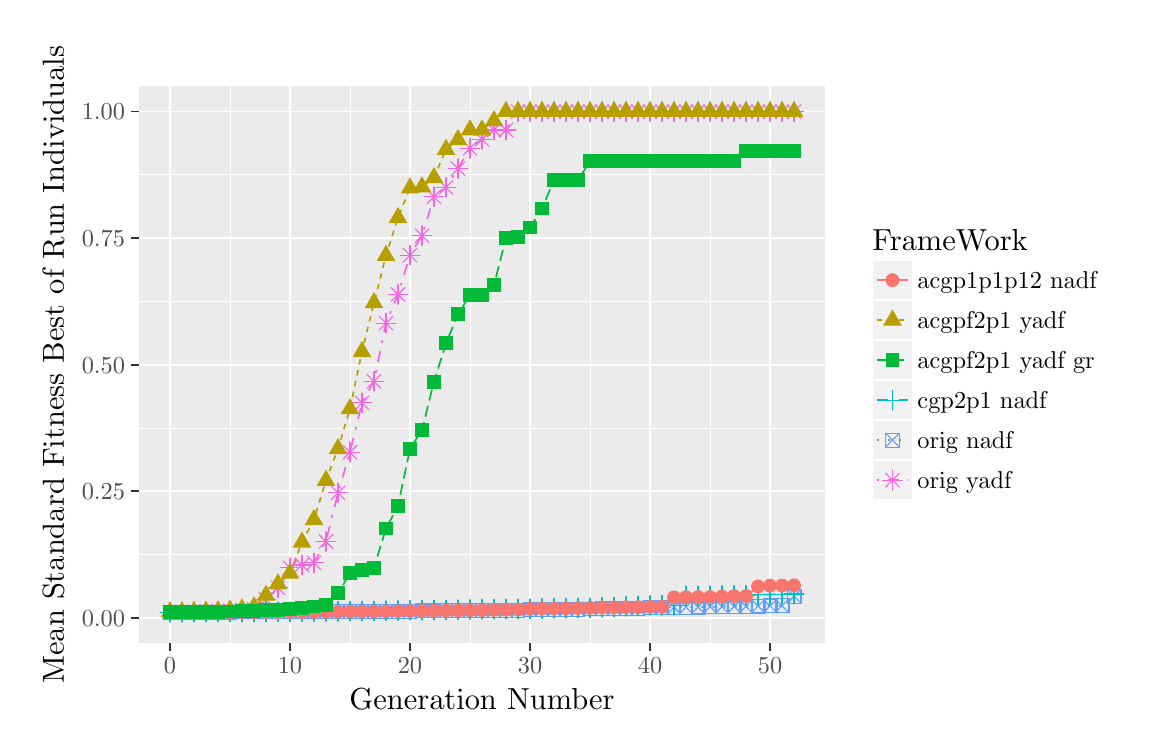
\begin{tikzpicture}[x=1pt,y=1pt]
\definecolor{fillColor}{RGB}{255,255,255}
\path[use as bounding box,fill=fillColor,fill opacity=0.00] (0,0) rectangle (397.48,252.94);
\begin{scope}
\path[clip] (  0.00,  0.00) rectangle (397.48,252.94);
\definecolor{drawColor}{RGB}{255,255,255}
\definecolor{fillColor}{RGB}{255,255,255}

\path[draw=drawColor,line width= 0.6pt,line join=round,line cap=round,fill=fillColor] (  0.00,  0.00) rectangle (397.48,252.95);
\end{scope}
\begin{scope}
\path[clip] ( 40.14, 30.56) rectangle (288.20,231.75);
\definecolor{fillColor}{gray}{0.92}

\path[fill=fillColor] ( 40.14, 30.56) rectangle (288.20,231.75);
\definecolor{drawColor}{RGB}{255,255,255}

\path[draw=drawColor,line width= 0.3pt,line join=round] ( 40.14, 62.57) --
	(288.20, 62.57);

\path[draw=drawColor,line width= 0.3pt,line join=round] ( 40.14,108.29) --
	(288.20,108.29);

\path[draw=drawColor,line width= 0.3pt,line join=round] ( 40.14,154.02) --
	(288.20,154.02);

\path[draw=drawColor,line width= 0.3pt,line join=round] ( 40.14,199.75) --
	(288.20,199.75);

\path[draw=drawColor,line width= 0.3pt,line join=round] ( 73.10, 30.56) --
	( 73.10,231.75);

\path[draw=drawColor,line width= 0.3pt,line join=round] (116.47, 30.56) --
	(116.47,231.75);

\path[draw=drawColor,line width= 0.3pt,line join=round] (159.83, 30.56) --
	(159.83,231.75);

\path[draw=drawColor,line width= 0.3pt,line join=round] (203.20, 30.56) --
	(203.20,231.75);

\path[draw=drawColor,line width= 0.3pt,line join=round] (246.57, 30.56) --
	(246.57,231.75);

\path[draw=drawColor,line width= 0.6pt,line join=round] ( 40.14, 39.70) --
	(288.20, 39.70);

\path[draw=drawColor,line width= 0.6pt,line join=round] ( 40.14, 85.43) --
	(288.20, 85.43);

\path[draw=drawColor,line width= 0.6pt,line join=round] ( 40.14,131.16) --
	(288.20,131.16);

\path[draw=drawColor,line width= 0.6pt,line join=round] ( 40.14,176.88) --
	(288.20,176.88);

\path[draw=drawColor,line width= 0.6pt,line join=round] ( 40.14,222.61) --
	(288.20,222.61);

\path[draw=drawColor,line width= 0.6pt,line join=round] ( 51.41, 30.56) --
	( 51.41,231.75);

\path[draw=drawColor,line width= 0.6pt,line join=round] ( 94.78, 30.56) --
	( 94.78,231.75);

\path[draw=drawColor,line width= 0.6pt,line join=round] (138.15, 30.56) --
	(138.15,231.75);

\path[draw=drawColor,line width= 0.6pt,line join=round] (181.52, 30.56) --
	(181.52,231.75);

\path[draw=drawColor,line width= 0.6pt,line join=round] (224.88, 30.56) --
	(224.88,231.75);

\path[draw=drawColor,line width= 0.6pt,line join=round] (268.25, 30.56) --
	(268.25,231.75);
\definecolor{drawColor}{RGB}{248,118,109}

\path[draw=drawColor,line width= 0.6pt,line join=round] ( 51.41, 41.70) --
	( 55.75, 41.72) --
	( 60.09, 41.72) --
	( 64.42, 41.72) --
	( 68.76, 41.73) --
	( 73.10, 41.75) --
	( 77.43, 41.76) --
	( 81.77, 41.77) --
	( 86.11, 41.77) --
	( 90.44, 41.78) --
	( 94.78, 41.79) --
	( 99.12, 41.80) --
	(103.45, 41.82) --
	(107.79, 41.86) --
	(112.13, 41.89) --
	(116.47, 41.95) --
	(120.80, 41.98) --
	(125.14, 42.00) --
	(129.48, 42.05) --
	(133.81, 42.10) --
	(138.15, 42.14) --
	(142.49, 42.19) --
	(146.82, 42.21) --
	(151.16, 42.32) --
	(155.50, 42.38) --
	(159.83, 42.43) --
	(164.17, 42.48) --
	(168.51, 42.56) --
	(172.84, 42.62) --
	(177.18, 42.67) --
	(181.52, 42.94) --
	(185.85, 43.00) --
	(190.19, 43.05) --
	(194.53, 43.11) --
	(198.86, 43.22) --
	(203.20, 43.31) --
	(207.54, 43.42) --
	(211.87, 43.43) --
	(216.21, 43.50) --
	(220.55, 43.54) --
	(224.88, 43.64) --
	(229.22, 43.67) --
	(233.56, 47.08) --
	(237.89, 47.12) --
	(242.23, 47.16) --
	(246.57, 47.18) --
	(250.90, 47.38) --
	(255.24, 47.53) --
	(259.58, 47.60) --
	(263.91, 51.04) --
	(268.25, 51.33) --
	(272.59, 51.35) --
	(276.92, 51.44);
\definecolor{drawColor}{RGB}{183,159,0}

\path[draw=drawColor,line width= 0.6pt,dash pattern=on 2pt off 2pt ,line join=round] ( 51.41, 41.77) --
	( 55.75, 41.82) --
	( 60.09, 41.97) --
	( 64.42, 42.08) --
	( 68.76, 42.22) --
	( 73.10, 42.45) --
	( 77.43, 42.81) --
	( 81.77, 43.62) --
	( 86.11, 47.80) --
	( 90.44, 51.91) --
	( 94.78, 55.77) --
	( 99.12, 67.02) --
	(103.45, 75.14) --
	(107.79, 89.32) --
	(112.13,100.76) --
	(116.47,115.21) --
	(120.80,135.86) --
	(125.14,153.54) --
	(129.48,170.57) --
	(133.81,184.28) --
	(138.15,194.99) --
	(142.49,195.39) --
	(146.82,198.74) --
	(151.16,208.93) --
	(155.50,212.47) --
	(159.83,215.96) --
	(164.17,215.96) --
	(168.51,219.28) --
	(172.84,222.61) --
	(177.18,222.61) --
	(181.52,222.61) --
	(185.85,222.61) --
	(190.19,222.61) --
	(194.53,222.61) --
	(198.86,222.61) --
	(203.20,222.61) --
	(207.54,222.61) --
	(211.87,222.61) --
	(216.21,222.61) --
	(220.55,222.61) --
	(224.88,222.61) --
	(229.22,222.61) --
	(233.56,222.61) --
	(237.89,222.61) --
	(242.23,222.61) --
	(246.57,222.61) --
	(250.90,222.61) --
	(255.24,222.61) --
	(259.58,222.61) --
	(263.91,222.61) --
	(268.25,222.61) --
	(272.59,222.61) --
	(276.92,222.61);
\definecolor{drawColor}{RGB}{0,186,56}

\path[draw=drawColor,line width= 0.6pt,dash pattern=on 4pt off 2pt ,line join=round] ( 51.41, 41.72) --
	( 55.75, 41.78) --
	( 60.09, 41.80) --
	( 64.42, 41.85) --
	( 68.76, 41.87) --
	( 73.10, 41.96) --
	( 77.43, 42.10) --
	( 81.77, 42.27) --
	( 86.11, 42.43) --
	( 90.44, 42.59) --
	( 94.78, 42.89) --
	( 99.12, 43.27) --
	(103.45, 43.79) --
	(107.79, 44.36) --
	(112.13, 48.54) --
	(116.47, 55.75) --
	(120.80, 56.88) --
	(125.14, 57.84) --
	(129.48, 71.98) --
	(133.81, 80.03) --
	(138.15,100.78) --
	(142.49,107.58) --
	(146.82,125.04) --
	(151.16,138.91) --
	(155.50,149.39) --
	(159.83,156.27) --
	(164.17,156.39) --
	(168.51,160.03) --
	(172.84,176.94) --
	(177.18,177.24) --
	(181.52,180.74) --
	(185.85,187.58) --
	(190.19,197.94) --
	(194.53,197.94) --
	(198.86,197.94) --
	(203.20,204.61) --
	(207.54,204.61) --
	(211.87,204.63) --
	(216.21,204.63) --
	(220.55,204.66) --
	(224.88,204.66) --
	(229.22,204.68) --
	(233.56,204.68) --
	(237.89,204.74) --
	(242.23,204.74) --
	(246.57,204.80) --
	(250.90,204.80) --
	(255.24,204.80) --
	(259.58,208.28) --
	(263.91,208.28) --
	(268.25,208.28) --
	(272.59,208.44) --
	(276.92,208.44);
\definecolor{drawColor}{RGB}{0,191,196}

\path[draw=drawColor,line width= 0.6pt,dash pattern=on 4pt off 4pt ,line join=round] ( 51.41, 41.71) --
	( 55.75, 41.73) --
	( 60.09, 41.73) --
	( 64.42, 41.77) --
	( 68.76, 41.78) --
	( 73.10, 41.78) --
	( 77.43, 41.80) --
	( 81.77, 41.82) --
	( 86.11, 41.85) --
	( 90.44, 41.87) --
	( 94.78, 41.88) --
	( 99.12, 41.92) --
	(103.45, 41.94) --
	(107.79, 41.98) --
	(112.13, 42.03) --
	(116.47, 42.07) --
	(120.80, 42.12) --
	(125.14, 42.17) --
	(129.48, 42.30) --
	(133.81, 42.32) --
	(138.15, 42.40) --
	(142.49, 42.43) --
	(146.82, 42.51) --
	(151.16, 42.55) --
	(155.50, 42.63) --
	(159.83, 42.72) --
	(164.17, 42.77) --
	(168.51, 42.81) --
	(172.84, 42.89) --
	(177.18, 42.91) --
	(181.52, 42.96) --
	(185.85, 43.07) --
	(190.19, 43.14) --
	(194.53, 43.17) --
	(198.86, 43.26) --
	(203.20, 43.31) --
	(207.54, 43.49) --
	(211.87, 43.62) --
	(216.21, 43.85) --
	(220.55, 44.02) --
	(224.88, 44.17) --
	(229.22, 44.19) --
	(233.56, 44.20) --
	(237.89, 47.57) --
	(242.23, 47.62) --
	(246.57, 47.66) --
	(250.90, 47.75) --
	(255.24, 47.76) --
	(259.58, 47.90) --
	(263.91, 47.98) --
	(268.25, 48.12) --
	(272.59, 48.21) --
	(276.92, 48.31);
\definecolor{drawColor}{RGB}{97,156,255}

\path[draw=drawColor,line width= 0.6pt,dash pattern=on 1pt off 3pt ,line join=round] ( 51.41, 41.69) --
	( 55.75, 41.72) --
	( 60.09, 41.73) --
	( 64.42, 41.73) --
	( 68.76, 41.76) --
	( 73.10, 41.78) --
	( 77.43, 41.79) --
	( 81.77, 41.80) --
	( 86.11, 41.81) --
	( 90.44, 41.82) --
	( 94.78, 41.84) --
	( 99.12, 41.86) --
	(103.45, 41.88) --
	(107.79, 41.89) --
	(112.13, 41.94) --
	(116.47, 41.94) --
	(120.80, 42.00) --
	(125.14, 42.03) --
	(129.48, 42.06) --
	(133.81, 42.07) --
	(138.15, 42.10) --
	(142.49, 42.18) --
	(146.82, 42.19) --
	(151.16, 42.22) --
	(155.50, 42.25) --
	(159.83, 42.26) --
	(164.17, 42.30) --
	(168.51, 42.36) --
	(172.84, 42.39) --
	(177.18, 42.46) --
	(181.52, 42.53) --
	(185.85, 42.64) --
	(190.19, 42.75) --
	(194.53, 42.77) --
	(198.86, 42.79) --
	(203.20, 42.88) --
	(207.54, 43.00) --
	(211.87, 43.07) --
	(216.21, 43.13) --
	(220.55, 43.15) --
	(224.88, 43.40) --
	(229.22, 43.42) --
	(233.56, 43.49) --
	(237.89, 43.54) --
	(242.23, 43.58) --
	(246.57, 43.70) --
	(250.90, 43.70) --
	(255.24, 43.80) --
	(259.58, 43.82) --
	(263.91, 43.94) --
	(268.25, 43.98) --
	(272.59, 44.01) --
	(276.92, 47.50);
\definecolor{drawColor}{RGB}{245,100,227}

\path[draw=drawColor,line width= 0.6pt,dash pattern=on 1pt off 3pt on 4pt off 3pt ,line join=round] ( 51.41, 41.73) --
	( 55.75, 41.80) --
	( 60.09, 41.89) --
	( 64.42, 41.97) --
	( 68.76, 42.09) --
	( 73.10, 42.25) --
	( 77.43, 42.42) --
	( 81.77, 42.75) --
	( 86.11, 46.39) --
	( 90.44, 50.50) --
	( 94.78, 57.78) --
	( 99.12, 58.79) --
	(103.45, 59.56) --
	(107.79, 67.27) --
	(112.13, 84.84) --
	(116.47, 99.50) --
	(120.80,117.35) --
	(125.14,125.14) --
	(129.48,146.17) --
	(133.81,156.53) --
	(138.15,170.75) --
	(142.49,177.81) --
	(146.82,191.83) --
	(151.16,195.21) --
	(155.50,202.02) --
	(159.83,209.31) --
	(164.17,212.63) --
	(168.51,215.96) --
	(172.84,215.96) --
	(177.18,222.61) --
	(181.52,222.61) --
	(185.85,222.61) --
	(190.19,222.61) --
	(194.53,222.61) --
	(198.86,222.61) --
	(203.20,222.61) --
	(207.54,222.61) --
	(211.87,222.61) --
	(216.21,222.61) --
	(220.55,222.61) --
	(224.88,222.61) --
	(229.22,222.61) --
	(233.56,222.61) --
	(237.89,222.61) --
	(242.23,222.61) --
	(246.57,222.61) --
	(250.90,222.61) --
	(255.24,222.61) --
	(259.58,222.61) --
	(263.91,222.61) --
	(268.25,222.61) --
	(272.59,222.61) --
	(276.92,222.61);
\definecolor{drawColor}{RGB}{97,156,255}

\path[draw=drawColor,line width= 0.4pt,line join=round,line cap=round] ( 48.92, 39.19) rectangle ( 53.91, 44.19);

\path[draw=drawColor,line width= 0.4pt,line join=round,line cap=round] ( 48.92, 39.19) -- ( 53.91, 44.19);

\path[draw=drawColor,line width= 0.4pt,line join=round,line cap=round] ( 48.92, 44.19) -- ( 53.91, 39.19);

\path[draw=drawColor,line width= 0.4pt,line join=round,line cap=round] ( 53.25, 39.22) rectangle ( 58.25, 44.22);

\path[draw=drawColor,line width= 0.4pt,line join=round,line cap=round] ( 53.25, 39.22) -- ( 58.25, 44.22);

\path[draw=drawColor,line width= 0.4pt,line join=round,line cap=round] ( 53.25, 44.22) -- ( 58.25, 39.22);

\path[draw=drawColor,line width= 0.4pt,line join=round,line cap=round] ( 57.59, 39.23) rectangle ( 62.59, 44.22);

\path[draw=drawColor,line width= 0.4pt,line join=round,line cap=round] ( 57.59, 39.23) -- ( 62.59, 44.22);

\path[draw=drawColor,line width= 0.4pt,line join=round,line cap=round] ( 57.59, 44.22) -- ( 62.59, 39.23);

\path[draw=drawColor,line width= 0.4pt,line join=round,line cap=round] ( 61.93, 39.23) rectangle ( 66.92, 44.23);

\path[draw=drawColor,line width= 0.4pt,line join=round,line cap=round] ( 61.93, 39.23) -- ( 66.92, 44.23);

\path[draw=drawColor,line width= 0.4pt,line join=round,line cap=round] ( 61.93, 44.23) -- ( 66.92, 39.23);

\path[draw=drawColor,line width= 0.4pt,line join=round,line cap=round] ( 66.26, 39.26) rectangle ( 71.26, 44.25);

\path[draw=drawColor,line width= 0.4pt,line join=round,line cap=round] ( 66.26, 39.26) -- ( 71.26, 44.25);

\path[draw=drawColor,line width= 0.4pt,line join=round,line cap=round] ( 66.26, 44.25) -- ( 71.26, 39.26);

\path[draw=drawColor,line width= 0.4pt,line join=round,line cap=round] ( 70.60, 39.28) rectangle ( 75.60, 44.27);

\path[draw=drawColor,line width= 0.4pt,line join=round,line cap=round] ( 70.60, 39.28) -- ( 75.60, 44.27);

\path[draw=drawColor,line width= 0.4pt,line join=round,line cap=round] ( 70.60, 44.27) -- ( 75.60, 39.28);

\path[draw=drawColor,line width= 0.4pt,line join=round,line cap=round] ( 74.94, 39.29) rectangle ( 79.93, 44.29);

\path[draw=drawColor,line width= 0.4pt,line join=round,line cap=round] ( 74.94, 39.29) -- ( 79.93, 44.29);

\path[draw=drawColor,line width= 0.4pt,line join=round,line cap=round] ( 74.94, 44.29) -- ( 79.93, 39.29);

\path[draw=drawColor,line width= 0.4pt,line join=round,line cap=round] ( 79.27, 39.30) rectangle ( 84.27, 44.30);

\path[draw=drawColor,line width= 0.4pt,line join=round,line cap=round] ( 79.27, 39.30) -- ( 84.27, 44.30);

\path[draw=drawColor,line width= 0.4pt,line join=round,line cap=round] ( 79.27, 44.30) -- ( 84.27, 39.30);

\path[draw=drawColor,line width= 0.4pt,line join=round,line cap=round] ( 83.61, 39.31) rectangle ( 88.61, 44.31);

\path[draw=drawColor,line width= 0.4pt,line join=round,line cap=round] ( 83.61, 39.31) -- ( 88.61, 44.31);

\path[draw=drawColor,line width= 0.4pt,line join=round,line cap=round] ( 83.61, 44.31) -- ( 88.61, 39.31);

\path[draw=drawColor,line width= 0.4pt,line join=round,line cap=round] ( 87.95, 39.32) rectangle ( 92.94, 44.31);

\path[draw=drawColor,line width= 0.4pt,line join=round,line cap=round] ( 87.95, 39.32) -- ( 92.94, 44.31);

\path[draw=drawColor,line width= 0.4pt,line join=round,line cap=round] ( 87.95, 44.31) -- ( 92.94, 39.32);

\path[draw=drawColor,line width= 0.4pt,line join=round,line cap=round] ( 92.28, 39.34) rectangle ( 97.28, 44.33);

\path[draw=drawColor,line width= 0.4pt,line join=round,line cap=round] ( 92.28, 39.34) -- ( 97.28, 44.33);

\path[draw=drawColor,line width= 0.4pt,line join=round,line cap=round] ( 92.28, 44.33) -- ( 97.28, 39.34);

\path[draw=drawColor,line width= 0.4pt,line join=round,line cap=round] ( 96.62, 39.37) rectangle (101.62, 44.36);

\path[draw=drawColor,line width= 0.4pt,line join=round,line cap=round] ( 96.62, 39.37) -- (101.62, 44.36);

\path[draw=drawColor,line width= 0.4pt,line join=round,line cap=round] ( 96.62, 44.36) -- (101.62, 39.37);

\path[draw=drawColor,line width= 0.4pt,line join=round,line cap=round] (100.96, 39.38) rectangle (105.95, 44.37);

\path[draw=drawColor,line width= 0.4pt,line join=round,line cap=round] (100.96, 39.38) -- (105.95, 44.37);

\path[draw=drawColor,line width= 0.4pt,line join=round,line cap=round] (100.96, 44.37) -- (105.95, 39.38);

\path[draw=drawColor,line width= 0.4pt,line join=round,line cap=round] (105.29, 39.40) rectangle (110.29, 44.39);

\path[draw=drawColor,line width= 0.4pt,line join=round,line cap=round] (105.29, 39.40) -- (110.29, 44.39);

\path[draw=drawColor,line width= 0.4pt,line join=round,line cap=round] (105.29, 44.39) -- (110.29, 39.40);

\path[draw=drawColor,line width= 0.4pt,line join=round,line cap=round] (109.63, 39.44) rectangle (114.63, 44.43);

\path[draw=drawColor,line width= 0.4pt,line join=round,line cap=round] (109.63, 39.44) -- (114.63, 44.43);

\path[draw=drawColor,line width= 0.4pt,line join=round,line cap=round] (109.63, 44.43) -- (114.63, 39.44);

\path[draw=drawColor,line width= 0.4pt,line join=round,line cap=round] (113.97, 39.44) rectangle (118.96, 44.44);

\path[draw=drawColor,line width= 0.4pt,line join=round,line cap=round] (113.97, 39.44) -- (118.96, 44.44);

\path[draw=drawColor,line width= 0.4pt,line join=round,line cap=round] (113.97, 44.44) -- (118.96, 39.44);

\path[draw=drawColor,line width= 0.4pt,line join=round,line cap=round] (118.30, 39.50) rectangle (123.30, 44.49);

\path[draw=drawColor,line width= 0.4pt,line join=round,line cap=round] (118.30, 39.50) -- (123.30, 44.49);

\path[draw=drawColor,line width= 0.4pt,line join=round,line cap=round] (118.30, 44.49) -- (123.30, 39.50);

\path[draw=drawColor,line width= 0.4pt,line join=round,line cap=round] (122.64, 39.54) rectangle (127.64, 44.53);

\path[draw=drawColor,line width= 0.4pt,line join=round,line cap=round] (122.64, 39.54) -- (127.64, 44.53);

\path[draw=drawColor,line width= 0.4pt,line join=round,line cap=round] (122.64, 44.53) -- (127.64, 39.54);

\path[draw=drawColor,line width= 0.4pt,line join=round,line cap=round] (126.98, 39.56) rectangle (131.97, 44.56);

\path[draw=drawColor,line width= 0.4pt,line join=round,line cap=round] (126.98, 39.56) -- (131.97, 44.56);

\path[draw=drawColor,line width= 0.4pt,line join=round,line cap=round] (126.98, 44.56) -- (131.97, 39.56);

\path[draw=drawColor,line width= 0.4pt,line join=round,line cap=round] (131.31, 39.57) rectangle (136.31, 44.57);

\path[draw=drawColor,line width= 0.4pt,line join=round,line cap=round] (131.31, 39.57) -- (136.31, 44.57);

\path[draw=drawColor,line width= 0.4pt,line join=round,line cap=round] (131.31, 44.57) -- (136.31, 39.57);

\path[draw=drawColor,line width= 0.4pt,line join=round,line cap=round] (135.65, 39.60) rectangle (140.65, 44.59);

\path[draw=drawColor,line width= 0.4pt,line join=round,line cap=round] (135.65, 39.60) -- (140.65, 44.59);

\path[draw=drawColor,line width= 0.4pt,line join=round,line cap=round] (135.65, 44.59) -- (140.65, 39.60);

\path[draw=drawColor,line width= 0.4pt,line join=round,line cap=round] (139.99, 39.68) rectangle (144.98, 44.68);

\path[draw=drawColor,line width= 0.4pt,line join=round,line cap=round] (139.99, 39.68) -- (144.98, 44.68);

\path[draw=drawColor,line width= 0.4pt,line join=round,line cap=round] (139.99, 44.68) -- (144.98, 39.68);

\path[draw=drawColor,line width= 0.4pt,line join=round,line cap=round] (144.32, 39.69) rectangle (149.32, 44.68);

\path[draw=drawColor,line width= 0.4pt,line join=round,line cap=round] (144.32, 39.69) -- (149.32, 44.68);

\path[draw=drawColor,line width= 0.4pt,line join=round,line cap=round] (144.32, 44.68) -- (149.32, 39.69);

\path[draw=drawColor,line width= 0.4pt,line join=round,line cap=round] (148.66, 39.72) rectangle (153.66, 44.71);

\path[draw=drawColor,line width= 0.4pt,line join=round,line cap=round] (148.66, 39.72) -- (153.66, 44.71);

\path[draw=drawColor,line width= 0.4pt,line join=round,line cap=round] (148.66, 44.71) -- (153.66, 39.72);

\path[draw=drawColor,line width= 0.4pt,line join=round,line cap=round] (153.00, 39.75) rectangle (157.99, 44.75);

\path[draw=drawColor,line width= 0.4pt,line join=round,line cap=round] (153.00, 39.75) -- (157.99, 44.75);

\path[draw=drawColor,line width= 0.4pt,line join=round,line cap=round] (153.00, 44.75) -- (157.99, 39.75);

\path[draw=drawColor,line width= 0.4pt,line join=round,line cap=round] (157.33, 39.76) rectangle (162.33, 44.76);

\path[draw=drawColor,line width= 0.4pt,line join=round,line cap=round] (157.33, 39.76) -- (162.33, 44.76);

\path[draw=drawColor,line width= 0.4pt,line join=round,line cap=round] (157.33, 44.76) -- (162.33, 39.76);

\path[draw=drawColor,line width= 0.4pt,line join=round,line cap=round] (161.67, 39.80) rectangle (166.67, 44.80);

\path[draw=drawColor,line width= 0.4pt,line join=round,line cap=round] (161.67, 39.80) -- (166.67, 44.80);

\path[draw=drawColor,line width= 0.4pt,line join=round,line cap=round] (161.67, 44.80) -- (166.67, 39.80);

\path[draw=drawColor,line width= 0.4pt,line join=round,line cap=round] (166.01, 39.86) rectangle (171.00, 44.86);

\path[draw=drawColor,line width= 0.4pt,line join=round,line cap=round] (166.01, 39.86) -- (171.00, 44.86);

\path[draw=drawColor,line width= 0.4pt,line join=round,line cap=round] (166.01, 44.86) -- (171.00, 39.86);

\path[draw=drawColor,line width= 0.4pt,line join=round,line cap=round] (170.35, 39.90) rectangle (175.34, 44.89);

\path[draw=drawColor,line width= 0.4pt,line join=round,line cap=round] (170.35, 39.90) -- (175.34, 44.89);

\path[draw=drawColor,line width= 0.4pt,line join=round,line cap=round] (170.35, 44.89) -- (175.34, 39.90);

\path[draw=drawColor,line width= 0.4pt,line join=round,line cap=round] (174.68, 39.96) rectangle (179.68, 44.96);

\path[draw=drawColor,line width= 0.4pt,line join=round,line cap=round] (174.68, 39.96) -- (179.68, 44.96);

\path[draw=drawColor,line width= 0.4pt,line join=round,line cap=round] (174.68, 44.96) -- (179.68, 39.96);

\path[draw=drawColor,line width= 0.4pt,line join=round,line cap=round] (179.02, 40.03) rectangle (184.01, 45.03);

\path[draw=drawColor,line width= 0.4pt,line join=round,line cap=round] (179.02, 40.03) -- (184.01, 45.03);

\path[draw=drawColor,line width= 0.4pt,line join=round,line cap=round] (179.02, 45.03) -- (184.01, 40.03);

\path[draw=drawColor,line width= 0.4pt,line join=round,line cap=round] (183.36, 40.14) rectangle (188.35, 45.14);

\path[draw=drawColor,line width= 0.4pt,line join=round,line cap=round] (183.36, 40.14) -- (188.35, 45.14);

\path[draw=drawColor,line width= 0.4pt,line join=round,line cap=round] (183.36, 45.14) -- (188.35, 40.14);

\path[draw=drawColor,line width= 0.4pt,line join=round,line cap=round] (187.69, 40.25) rectangle (192.69, 45.25);

\path[draw=drawColor,line width= 0.4pt,line join=round,line cap=round] (187.69, 40.25) -- (192.69, 45.25);

\path[draw=drawColor,line width= 0.4pt,line join=round,line cap=round] (187.69, 45.25) -- (192.69, 40.25);

\path[draw=drawColor,line width= 0.4pt,line join=round,line cap=round] (192.03, 40.27) rectangle (197.02, 45.27);

\path[draw=drawColor,line width= 0.4pt,line join=round,line cap=round] (192.03, 40.27) -- (197.02, 45.27);

\path[draw=drawColor,line width= 0.4pt,line join=round,line cap=round] (192.03, 45.27) -- (197.02, 40.27);

\path[draw=drawColor,line width= 0.4pt,line join=round,line cap=round] (196.37, 40.29) rectangle (201.36, 45.29);

\path[draw=drawColor,line width= 0.4pt,line join=round,line cap=round] (196.37, 40.29) -- (201.36, 45.29);

\path[draw=drawColor,line width= 0.4pt,line join=round,line cap=round] (196.37, 45.29) -- (201.36, 40.29);

\path[draw=drawColor,line width= 0.4pt,line join=round,line cap=round] (200.70, 40.39) rectangle (205.70, 45.38);

\path[draw=drawColor,line width= 0.4pt,line join=round,line cap=round] (200.70, 40.39) -- (205.70, 45.38);

\path[draw=drawColor,line width= 0.4pt,line join=round,line cap=round] (200.70, 45.38) -- (205.70, 40.39);

\path[draw=drawColor,line width= 0.4pt,line join=round,line cap=round] (205.04, 40.50) rectangle (210.03, 45.50);

\path[draw=drawColor,line width= 0.4pt,line join=round,line cap=round] (205.04, 40.50) -- (210.03, 45.50);

\path[draw=drawColor,line width= 0.4pt,line join=round,line cap=round] (205.04, 45.50) -- (210.03, 40.50);

\path[draw=drawColor,line width= 0.4pt,line join=round,line cap=round] (209.38, 40.57) rectangle (214.37, 45.57);

\path[draw=drawColor,line width= 0.4pt,line join=round,line cap=round] (209.38, 40.57) -- (214.37, 45.57);

\path[draw=drawColor,line width= 0.4pt,line join=round,line cap=round] (209.38, 45.57) -- (214.37, 40.57);

\path[draw=drawColor,line width= 0.4pt,line join=round,line cap=round] (213.71, 40.63) rectangle (218.71, 45.63);

\path[draw=drawColor,line width= 0.4pt,line join=round,line cap=round] (213.71, 40.63) -- (218.71, 45.63);

\path[draw=drawColor,line width= 0.4pt,line join=round,line cap=round] (213.71, 45.63) -- (218.71, 40.63);

\path[draw=drawColor,line width= 0.4pt,line join=round,line cap=round] (218.05, 40.66) rectangle (223.04, 45.65);

\path[draw=drawColor,line width= 0.4pt,line join=round,line cap=round] (218.05, 40.66) -- (223.04, 45.65);

\path[draw=drawColor,line width= 0.4pt,line join=round,line cap=round] (218.05, 45.65) -- (223.04, 40.66);

\path[draw=drawColor,line width= 0.4pt,line join=round,line cap=round] (222.39, 40.90) rectangle (227.38, 45.89);

\path[draw=drawColor,line width= 0.4pt,line join=round,line cap=round] (222.39, 40.90) -- (227.38, 45.89);

\path[draw=drawColor,line width= 0.4pt,line join=round,line cap=round] (222.39, 45.89) -- (227.38, 40.90);

\path[draw=drawColor,line width= 0.4pt,line join=round,line cap=round] (226.72, 40.92) rectangle (231.72, 45.91);

\path[draw=drawColor,line width= 0.4pt,line join=round,line cap=round] (226.72, 40.92) -- (231.72, 45.91);

\path[draw=drawColor,line width= 0.4pt,line join=round,line cap=round] (226.72, 45.91) -- (231.72, 40.92);

\path[draw=drawColor,line width= 0.4pt,line join=round,line cap=round] (231.06, 41.00) rectangle (236.05, 45.99);

\path[draw=drawColor,line width= 0.4pt,line join=round,line cap=round] (231.06, 41.00) -- (236.05, 45.99);

\path[draw=drawColor,line width= 0.4pt,line join=round,line cap=round] (231.06, 45.99) -- (236.05, 41.00);

\path[draw=drawColor,line width= 0.4pt,line join=round,line cap=round] (235.40, 41.04) rectangle (240.39, 46.04);

\path[draw=drawColor,line width= 0.4pt,line join=round,line cap=round] (235.40, 41.04) -- (240.39, 46.04);

\path[draw=drawColor,line width= 0.4pt,line join=round,line cap=round] (235.40, 46.04) -- (240.39, 41.04);

\path[draw=drawColor,line width= 0.4pt,line join=round,line cap=round] (239.73, 41.08) rectangle (244.73, 46.08);

\path[draw=drawColor,line width= 0.4pt,line join=round,line cap=round] (239.73, 41.08) -- (244.73, 46.08);

\path[draw=drawColor,line width= 0.4pt,line join=round,line cap=round] (239.73, 46.08) -- (244.73, 41.08);

\path[draw=drawColor,line width= 0.4pt,line join=round,line cap=round] (244.07, 41.21) rectangle (249.06, 46.20);

\path[draw=drawColor,line width= 0.4pt,line join=round,line cap=round] (244.07, 41.21) -- (249.06, 46.20);

\path[draw=drawColor,line width= 0.4pt,line join=round,line cap=round] (244.07, 46.20) -- (249.06, 41.21);

\path[draw=drawColor,line width= 0.4pt,line join=round,line cap=round] (248.41, 41.21) rectangle (253.40, 46.20);

\path[draw=drawColor,line width= 0.4pt,line join=round,line cap=round] (248.41, 41.21) -- (253.40, 46.20);

\path[draw=drawColor,line width= 0.4pt,line join=round,line cap=round] (248.41, 46.20) -- (253.40, 41.21);

\path[draw=drawColor,line width= 0.4pt,line join=round,line cap=round] (252.74, 41.30) rectangle (257.74, 46.30);

\path[draw=drawColor,line width= 0.4pt,line join=round,line cap=round] (252.74, 41.30) -- (257.74, 46.30);

\path[draw=drawColor,line width= 0.4pt,line join=round,line cap=round] (252.74, 46.30) -- (257.74, 41.30);

\path[draw=drawColor,line width= 0.4pt,line join=round,line cap=round] (257.08, 41.32) rectangle (262.07, 46.32);

\path[draw=drawColor,line width= 0.4pt,line join=round,line cap=round] (257.08, 41.32) -- (262.07, 46.32);

\path[draw=drawColor,line width= 0.4pt,line join=round,line cap=round] (257.08, 46.32) -- (262.07, 41.32);

\path[draw=drawColor,line width= 0.4pt,line join=round,line cap=round] (261.42, 41.44) rectangle (266.41, 46.43);

\path[draw=drawColor,line width= 0.4pt,line join=round,line cap=round] (261.42, 41.44) -- (266.41, 46.43);

\path[draw=drawColor,line width= 0.4pt,line join=round,line cap=round] (261.42, 46.43) -- (266.41, 41.44);

\path[draw=drawColor,line width= 0.4pt,line join=round,line cap=round] (265.75, 41.48) rectangle (270.75, 46.48);

\path[draw=drawColor,line width= 0.4pt,line join=round,line cap=round] (265.75, 41.48) -- (270.75, 46.48);

\path[draw=drawColor,line width= 0.4pt,line join=round,line cap=round] (265.75, 46.48) -- (270.75, 41.48);

\path[draw=drawColor,line width= 0.4pt,line join=round,line cap=round] (270.09, 41.51) rectangle (275.09, 46.51);

\path[draw=drawColor,line width= 0.4pt,line join=round,line cap=round] (270.09, 41.51) -- (275.09, 46.51);

\path[draw=drawColor,line width= 0.4pt,line join=round,line cap=round] (270.09, 46.51) -- (275.09, 41.51);

\path[draw=drawColor,line width= 0.4pt,line join=round,line cap=round] (274.43, 45.00) rectangle (279.42, 50.00);

\path[draw=drawColor,line width= 0.4pt,line join=round,line cap=round] (274.43, 45.00) -- (279.42, 50.00);

\path[draw=drawColor,line width= 0.4pt,line join=round,line cap=round] (274.43, 50.00) -- (279.42, 45.00);
\definecolor{drawColor}{RGB}{245,100,227}

\path[draw=drawColor,line width= 0.4pt,line join=round,line cap=round] ( 48.92, 39.24) -- ( 53.91, 44.23);

\path[draw=drawColor,line width= 0.4pt,line join=round,line cap=round] ( 48.92, 44.23) -- ( 53.91, 39.24);

\path[draw=drawColor,line width= 0.4pt,line join=round,line cap=round] ( 47.88, 41.73) -- ( 54.95, 41.73);

\path[draw=drawColor,line width= 0.4pt,line join=round,line cap=round] ( 51.41, 38.20) -- ( 51.41, 45.27);

\path[draw=drawColor,line width= 0.4pt,line join=round,line cap=round] ( 53.25, 39.30) -- ( 58.25, 44.29);

\path[draw=drawColor,line width= 0.4pt,line join=round,line cap=round] ( 53.25, 44.29) -- ( 58.25, 39.30);

\path[draw=drawColor,line width= 0.4pt,line join=round,line cap=round] ( 52.22, 41.80) -- ( 59.28, 41.80);

\path[draw=drawColor,line width= 0.4pt,line join=round,line cap=round] ( 55.75, 38.26) -- ( 55.75, 45.33);

\path[draw=drawColor,line width= 0.4pt,line join=round,line cap=round] ( 57.59, 39.39) -- ( 62.59, 44.38);

\path[draw=drawColor,line width= 0.4pt,line join=round,line cap=round] ( 57.59, 44.38) -- ( 62.59, 39.39);

\path[draw=drawColor,line width= 0.4pt,line join=round,line cap=round] ( 56.56, 41.89) -- ( 63.62, 41.89);

\path[draw=drawColor,line width= 0.4pt,line join=round,line cap=round] ( 60.09, 38.35) -- ( 60.09, 45.42);

\path[draw=drawColor,line width= 0.4pt,line join=round,line cap=round] ( 61.93, 39.47) -- ( 66.92, 44.47);

\path[draw=drawColor,line width= 0.4pt,line join=round,line cap=round] ( 61.93, 44.47) -- ( 66.92, 39.47);

\path[draw=drawColor,line width= 0.4pt,line join=round,line cap=round] ( 60.89, 41.97) -- ( 67.96, 41.97);

\path[draw=drawColor,line width= 0.4pt,line join=round,line cap=round] ( 64.42, 38.44) -- ( 64.42, 45.50);

\path[draw=drawColor,line width= 0.4pt,line join=round,line cap=round] ( 66.26, 39.59) -- ( 71.26, 44.58);

\path[draw=drawColor,line width= 0.4pt,line join=round,line cap=round] ( 66.26, 44.58) -- ( 71.26, 39.59);

\path[draw=drawColor,line width= 0.4pt,line join=round,line cap=round] ( 65.23, 42.09) -- ( 72.29, 42.09);

\path[draw=drawColor,line width= 0.4pt,line join=round,line cap=round] ( 68.76, 38.55) -- ( 68.76, 45.62);

\path[draw=drawColor,line width= 0.4pt,line join=round,line cap=round] ( 70.60, 39.75) -- ( 75.60, 44.75);

\path[draw=drawColor,line width= 0.4pt,line join=round,line cap=round] ( 70.60, 44.75) -- ( 75.60, 39.75);

\path[draw=drawColor,line width= 0.4pt,line join=round,line cap=round] ( 69.57, 42.25) -- ( 76.63, 42.25);

\path[draw=drawColor,line width= 0.4pt,line join=round,line cap=round] ( 73.10, 38.72) -- ( 73.10, 45.78);

\path[draw=drawColor,line width= 0.4pt,line join=round,line cap=round] ( 74.94, 39.92) -- ( 79.93, 44.92);

\path[draw=drawColor,line width= 0.4pt,line join=round,line cap=round] ( 74.94, 44.92) -- ( 79.93, 39.92);

\path[draw=drawColor,line width= 0.4pt,line join=round,line cap=round] ( 73.90, 42.42) -- ( 80.97, 42.42);

\path[draw=drawColor,line width= 0.4pt,line join=round,line cap=round] ( 77.43, 38.89) -- ( 77.43, 45.95);

\path[draw=drawColor,line width= 0.4pt,line join=round,line cap=round] ( 79.27, 40.25) -- ( 84.27, 45.24);

\path[draw=drawColor,line width= 0.4pt,line join=round,line cap=round] ( 79.27, 45.24) -- ( 84.27, 40.25);

\path[draw=drawColor,line width= 0.4pt,line join=round,line cap=round] ( 78.24, 42.75) -- ( 85.30, 42.75);

\path[draw=drawColor,line width= 0.4pt,line join=round,line cap=round] ( 81.77, 39.21) -- ( 81.77, 46.28);

\path[draw=drawColor,line width= 0.4pt,line join=round,line cap=round] ( 83.61, 43.89) -- ( 88.61, 48.89);

\path[draw=drawColor,line width= 0.4pt,line join=round,line cap=round] ( 83.61, 48.89) -- ( 88.61, 43.89);

\path[draw=drawColor,line width= 0.4pt,line join=round,line cap=round] ( 82.58, 46.39) -- ( 89.64, 46.39);

\path[draw=drawColor,line width= 0.4pt,line join=round,line cap=round] ( 86.11, 42.86) -- ( 86.11, 49.92);

\path[draw=drawColor,line width= 0.4pt,line join=round,line cap=round] ( 87.95, 48.00) -- ( 92.94, 53.00);

\path[draw=drawColor,line width= 0.4pt,line join=round,line cap=round] ( 87.95, 53.00) -- ( 92.94, 48.00);

\path[draw=drawColor,line width= 0.4pt,line join=round,line cap=round] ( 86.91, 50.50) -- ( 93.98, 50.50);

\path[draw=drawColor,line width= 0.4pt,line join=round,line cap=round] ( 90.44, 46.97) -- ( 90.44, 54.03);

\path[draw=drawColor,line width= 0.4pt,line join=round,line cap=round] ( 92.28, 55.28) -- ( 97.28, 60.28);

\path[draw=drawColor,line width= 0.4pt,line join=round,line cap=round] ( 92.28, 60.28) -- ( 97.28, 55.28);

\path[draw=drawColor,line width= 0.4pt,line join=round,line cap=round] ( 91.25, 57.78) -- ( 98.31, 57.78);

\path[draw=drawColor,line width= 0.4pt,line join=round,line cap=round] ( 94.78, 54.25) -- ( 94.78, 61.31);

\path[draw=drawColor,line width= 0.4pt,line join=round,line cap=round] ( 96.62, 56.29) -- (101.62, 61.29);

\path[draw=drawColor,line width= 0.4pt,line join=round,line cap=round] ( 96.62, 61.29) -- (101.62, 56.29);

\path[draw=drawColor,line width= 0.4pt,line join=round,line cap=round] ( 95.59, 58.79) -- (102.65, 58.79);

\path[draw=drawColor,line width= 0.4pt,line join=round,line cap=round] ( 99.12, 55.26) -- ( 99.12, 62.32);

\path[draw=drawColor,line width= 0.4pt,line join=round,line cap=round] (100.96, 57.06) -- (105.95, 62.06);

\path[draw=drawColor,line width= 0.4pt,line join=round,line cap=round] (100.96, 62.06) -- (105.95, 57.06);

\path[draw=drawColor,line width= 0.4pt,line join=round,line cap=round] ( 99.92, 59.56) -- (106.99, 59.56);

\path[draw=drawColor,line width= 0.4pt,line join=round,line cap=round] (103.45, 56.03) -- (103.45, 63.09);

\path[draw=drawColor,line width= 0.4pt,line join=round,line cap=round] (105.29, 64.78) -- (110.29, 69.77);

\path[draw=drawColor,line width= 0.4pt,line join=round,line cap=round] (105.29, 69.77) -- (110.29, 64.78);

\path[draw=drawColor,line width= 0.4pt,line join=round,line cap=round] (104.26, 67.27) -- (111.32, 67.27);

\path[draw=drawColor,line width= 0.4pt,line join=round,line cap=round] (107.79, 63.74) -- (107.79, 70.81);

\path[draw=drawColor,line width= 0.4pt,line join=round,line cap=round] (109.63, 82.34) -- (114.63, 87.34);

\path[draw=drawColor,line width= 0.4pt,line join=round,line cap=round] (109.63, 87.34) -- (114.63, 82.34);

\path[draw=drawColor,line width= 0.4pt,line join=round,line cap=round] (108.60, 84.84) -- (115.66, 84.84);

\path[draw=drawColor,line width= 0.4pt,line join=round,line cap=round] (112.13, 81.31) -- (112.13, 88.37);

\path[draw=drawColor,line width= 0.4pt,line join=round,line cap=round] (113.97, 97.01) -- (118.96,102.00);

\path[draw=drawColor,line width= 0.4pt,line join=round,line cap=round] (113.97,102.00) -- (118.96, 97.01);

\path[draw=drawColor,line width= 0.4pt,line join=round,line cap=round] (112.93, 99.50) -- (120.00, 99.50);

\path[draw=drawColor,line width= 0.4pt,line join=round,line cap=round] (116.47, 95.97) -- (116.47,103.04);

\path[draw=drawColor,line width= 0.4pt,line join=round,line cap=round] (118.30,114.86) -- (123.30,119.85);

\path[draw=drawColor,line width= 0.4pt,line join=round,line cap=round] (118.30,119.85) -- (123.30,114.86);

\path[draw=drawColor,line width= 0.4pt,line join=round,line cap=round] (117.27,117.35) -- (124.33,117.35);

\path[draw=drawColor,line width= 0.4pt,line join=round,line cap=round] (120.80,113.82) -- (120.80,120.89);

\path[draw=drawColor,line width= 0.4pt,line join=round,line cap=round] (122.64,122.64) -- (127.64,127.64);

\path[draw=drawColor,line width= 0.4pt,line join=round,line cap=round] (122.64,127.64) -- (127.64,122.64);

\path[draw=drawColor,line width= 0.4pt,line join=round,line cap=round] (121.61,125.14) -- (128.67,125.14);

\path[draw=drawColor,line width= 0.4pt,line join=round,line cap=round] (125.14,121.61) -- (125.14,128.67);

\path[draw=drawColor,line width= 0.4pt,line join=round,line cap=round] (126.98,143.67) -- (131.97,148.67);

\path[draw=drawColor,line width= 0.4pt,line join=round,line cap=round] (126.98,148.67) -- (131.97,143.67);

\path[draw=drawColor,line width= 0.4pt,line join=round,line cap=round] (125.94,146.17) -- (133.01,146.17);

\path[draw=drawColor,line width= 0.4pt,line join=round,line cap=round] (129.48,142.64) -- (129.48,149.70);

\path[draw=drawColor,line width= 0.4pt,line join=round,line cap=round] (131.31,154.03) -- (136.31,159.02);

\path[draw=drawColor,line width= 0.4pt,line join=round,line cap=round] (131.31,159.02) -- (136.31,154.03);

\path[draw=drawColor,line width= 0.4pt,line join=round,line cap=round] (130.28,156.53) -- (137.34,156.53);

\path[draw=drawColor,line width= 0.4pt,line join=round,line cap=round] (133.81,152.99) -- (133.81,160.06);

\path[draw=drawColor,line width= 0.4pt,line join=round,line cap=round] (135.65,168.25) -- (140.65,173.24);

\path[draw=drawColor,line width= 0.4pt,line join=round,line cap=round] (135.65,173.24) -- (140.65,168.25);

\path[draw=drawColor,line width= 0.4pt,line join=round,line cap=round] (134.62,170.75) -- (141.68,170.75);

\path[draw=drawColor,line width= 0.4pt,line join=round,line cap=round] (138.15,167.21) -- (138.15,174.28);

\path[draw=drawColor,line width= 0.4pt,line join=round,line cap=round] (139.99,175.31) -- (144.98,180.31);

\path[draw=drawColor,line width= 0.4pt,line join=round,line cap=round] (139.99,180.31) -- (144.98,175.31);

\path[draw=drawColor,line width= 0.4pt,line join=round,line cap=round] (138.95,177.81) -- (146.02,177.81);

\path[draw=drawColor,line width= 0.4pt,line join=round,line cap=round] (142.49,174.28) -- (142.49,181.34);

\path[draw=drawColor,line width= 0.4pt,line join=round,line cap=round] (144.32,189.33) -- (149.32,194.33);

\path[draw=drawColor,line width= 0.4pt,line join=round,line cap=round] (144.32,194.33) -- (149.32,189.33);

\path[draw=drawColor,line width= 0.4pt,line join=round,line cap=round] (143.29,191.83) -- (150.35,191.83);

\path[draw=drawColor,line width= 0.4pt,line join=round,line cap=round] (146.82,188.30) -- (146.82,195.36);

\path[draw=drawColor,line width= 0.4pt,line join=round,line cap=round] (148.66,192.71) -- (153.66,197.71);

\path[draw=drawColor,line width= 0.4pt,line join=round,line cap=round] (148.66,197.71) -- (153.66,192.71);

\path[draw=drawColor,line width= 0.4pt,line join=round,line cap=round] (147.63,195.21) -- (154.69,195.21);

\path[draw=drawColor,line width= 0.4pt,line join=round,line cap=round] (151.16,191.68) -- (151.16,198.74);

\path[draw=drawColor,line width= 0.4pt,line join=round,line cap=round] (153.00,199.52) -- (157.99,204.52);

\path[draw=drawColor,line width= 0.4pt,line join=round,line cap=round] (153.00,204.52) -- (157.99,199.52);

\path[draw=drawColor,line width= 0.4pt,line join=round,line cap=round] (151.96,202.02) -- (159.03,202.02);

\path[draw=drawColor,line width= 0.4pt,line join=round,line cap=round] (155.50,198.49) -- (155.50,205.55);

\path[draw=drawColor,line width= 0.4pt,line join=round,line cap=round] (157.33,206.81) -- (162.33,211.80);

\path[draw=drawColor,line width= 0.4pt,line join=round,line cap=round] (157.33,211.80) -- (162.33,206.81);

\path[draw=drawColor,line width= 0.4pt,line join=round,line cap=round] (156.30,209.31) -- (163.36,209.31);

\path[draw=drawColor,line width= 0.4pt,line join=round,line cap=round] (159.83,205.77) -- (159.83,212.84);

\path[draw=drawColor,line width= 0.4pt,line join=round,line cap=round] (161.67,210.13) -- (166.67,215.13);

\path[draw=drawColor,line width= 0.4pt,line join=round,line cap=round] (161.67,215.13) -- (166.67,210.13);

\path[draw=drawColor,line width= 0.4pt,line join=round,line cap=round] (160.64,212.63) -- (167.70,212.63);

\path[draw=drawColor,line width= 0.4pt,line join=round,line cap=round] (164.17,209.10) -- (164.17,216.16);

\path[draw=drawColor,line width= 0.4pt,line join=round,line cap=round] (166.01,213.46) -- (171.00,218.46);

\path[draw=drawColor,line width= 0.4pt,line join=round,line cap=round] (166.01,218.46) -- (171.00,213.46);

\path[draw=drawColor,line width= 0.4pt,line join=round,line cap=round] (164.97,215.96) -- (172.04,215.96);

\path[draw=drawColor,line width= 0.4pt,line join=round,line cap=round] (168.51,212.43) -- (168.51,219.49);

\path[draw=drawColor,line width= 0.4pt,line join=round,line cap=round] (170.35,213.46) -- (175.34,218.46);

\path[draw=drawColor,line width= 0.4pt,line join=round,line cap=round] (170.35,218.46) -- (175.34,213.46);

\path[draw=drawColor,line width= 0.4pt,line join=round,line cap=round] (169.31,215.96) -- (176.37,215.96);

\path[draw=drawColor,line width= 0.4pt,line join=round,line cap=round] (172.84,212.43) -- (172.84,219.49);

\path[draw=drawColor,line width= 0.4pt,line join=round,line cap=round] (174.68,220.11) -- (179.68,225.11);

\path[draw=drawColor,line width= 0.4pt,line join=round,line cap=round] (174.68,225.11) -- (179.68,220.11);

\path[draw=drawColor,line width= 0.4pt,line join=round,line cap=round] (173.65,222.61) -- (180.71,222.61);

\path[draw=drawColor,line width= 0.4pt,line join=round,line cap=round] (177.18,219.08) -- (177.18,226.14);

\path[draw=drawColor,line width= 0.4pt,line join=round,line cap=round] (179.02,220.11) -- (184.01,225.11);

\path[draw=drawColor,line width= 0.4pt,line join=round,line cap=round] (179.02,225.11) -- (184.01,220.11);

\path[draw=drawColor,line width= 0.4pt,line join=round,line cap=round] (177.98,222.61) -- (185.05,222.61);

\path[draw=drawColor,line width= 0.4pt,line join=round,line cap=round] (181.52,219.08) -- (181.52,226.14);

\path[draw=drawColor,line width= 0.4pt,line join=round,line cap=round] (183.36,220.11) -- (188.35,225.11);

\path[draw=drawColor,line width= 0.4pt,line join=round,line cap=round] (183.36,225.11) -- (188.35,220.11);

\path[draw=drawColor,line width= 0.4pt,line join=round,line cap=round] (182.32,222.61) -- (189.39,222.61);

\path[draw=drawColor,line width= 0.4pt,line join=round,line cap=round] (185.85,219.08) -- (185.85,226.14);

\path[draw=drawColor,line width= 0.4pt,line join=round,line cap=round] (187.69,220.11) -- (192.69,225.11);

\path[draw=drawColor,line width= 0.4pt,line join=round,line cap=round] (187.69,225.11) -- (192.69,220.11);

\path[draw=drawColor,line width= 0.4pt,line join=round,line cap=round] (186.66,222.61) -- (193.72,222.61);

\path[draw=drawColor,line width= 0.4pt,line join=round,line cap=round] (190.19,219.08) -- (190.19,226.14);

\path[draw=drawColor,line width= 0.4pt,line join=round,line cap=round] (192.03,220.11) -- (197.02,225.11);

\path[draw=drawColor,line width= 0.4pt,line join=round,line cap=round] (192.03,225.11) -- (197.02,220.11);

\path[draw=drawColor,line width= 0.4pt,line join=round,line cap=round] (190.99,222.61) -- (198.06,222.61);

\path[draw=drawColor,line width= 0.4pt,line join=round,line cap=round] (194.53,219.08) -- (194.53,226.14);

\path[draw=drawColor,line width= 0.4pt,line join=round,line cap=round] (196.37,220.11) -- (201.36,225.11);

\path[draw=drawColor,line width= 0.4pt,line join=round,line cap=round] (196.37,225.11) -- (201.36,220.11);

\path[draw=drawColor,line width= 0.4pt,line join=round,line cap=round] (195.33,222.61) -- (202.40,222.61);

\path[draw=drawColor,line width= 0.4pt,line join=round,line cap=round] (198.86,219.08) -- (198.86,226.14);

\path[draw=drawColor,line width= 0.4pt,line join=round,line cap=round] (200.70,220.11) -- (205.70,225.11);

\path[draw=drawColor,line width= 0.4pt,line join=round,line cap=round] (200.70,225.11) -- (205.70,220.11);

\path[draw=drawColor,line width= 0.4pt,line join=round,line cap=round] (199.67,222.61) -- (206.73,222.61);

\path[draw=drawColor,line width= 0.4pt,line join=round,line cap=round] (203.20,219.08) -- (203.20,226.14);

\path[draw=drawColor,line width= 0.4pt,line join=round,line cap=round] (205.04,220.11) -- (210.03,225.11);

\path[draw=drawColor,line width= 0.4pt,line join=round,line cap=round] (205.04,225.11) -- (210.03,220.11);

\path[draw=drawColor,line width= 0.4pt,line join=round,line cap=round] (204.00,222.61) -- (211.07,222.61);

\path[draw=drawColor,line width= 0.4pt,line join=round,line cap=round] (207.54,219.08) -- (207.54,226.14);

\path[draw=drawColor,line width= 0.4pt,line join=round,line cap=round] (209.38,220.11) -- (214.37,225.11);

\path[draw=drawColor,line width= 0.4pt,line join=round,line cap=round] (209.38,225.11) -- (214.37,220.11);

\path[draw=drawColor,line width= 0.4pt,line join=round,line cap=round] (208.34,222.61) -- (215.41,222.61);

\path[draw=drawColor,line width= 0.4pt,line join=round,line cap=round] (211.87,219.08) -- (211.87,226.14);

\path[draw=drawColor,line width= 0.4pt,line join=round,line cap=round] (213.71,220.11) -- (218.71,225.11);

\path[draw=drawColor,line width= 0.4pt,line join=round,line cap=round] (213.71,225.11) -- (218.71,220.11);

\path[draw=drawColor,line width= 0.4pt,line join=round,line cap=round] (212.68,222.61) -- (219.74,222.61);

\path[draw=drawColor,line width= 0.4pt,line join=round,line cap=round] (216.21,219.08) -- (216.21,226.14);

\path[draw=drawColor,line width= 0.4pt,line join=round,line cap=round] (218.05,220.11) -- (223.04,225.11);

\path[draw=drawColor,line width= 0.4pt,line join=round,line cap=round] (218.05,225.11) -- (223.04,220.11);

\path[draw=drawColor,line width= 0.4pt,line join=round,line cap=round] (217.01,222.61) -- (224.08,222.61);

\path[draw=drawColor,line width= 0.4pt,line join=round,line cap=round] (220.55,219.08) -- (220.55,226.14);

\path[draw=drawColor,line width= 0.4pt,line join=round,line cap=round] (222.39,220.11) -- (227.38,225.11);

\path[draw=drawColor,line width= 0.4pt,line join=round,line cap=round] (222.39,225.11) -- (227.38,220.11);

\path[draw=drawColor,line width= 0.4pt,line join=round,line cap=round] (221.35,222.61) -- (228.42,222.61);

\path[draw=drawColor,line width= 0.4pt,line join=round,line cap=round] (224.88,219.08) -- (224.88,226.14);

\path[draw=drawColor,line width= 0.4pt,line join=round,line cap=round] (226.72,220.11) -- (231.72,225.11);

\path[draw=drawColor,line width= 0.4pt,line join=round,line cap=round] (226.72,225.11) -- (231.72,220.11);

\path[draw=drawColor,line width= 0.4pt,line join=round,line cap=round] (225.69,222.61) -- (232.75,222.61);

\path[draw=drawColor,line width= 0.4pt,line join=round,line cap=round] (229.22,219.08) -- (229.22,226.14);

\path[draw=drawColor,line width= 0.4pt,line join=round,line cap=round] (231.06,220.11) -- (236.05,225.11);

\path[draw=drawColor,line width= 0.4pt,line join=round,line cap=round] (231.06,225.11) -- (236.05,220.11);

\path[draw=drawColor,line width= 0.4pt,line join=round,line cap=round] (230.02,222.61) -- (237.09,222.61);

\path[draw=drawColor,line width= 0.4pt,line join=round,line cap=round] (233.56,219.08) -- (233.56,226.14);

\path[draw=drawColor,line width= 0.4pt,line join=round,line cap=round] (235.40,220.11) -- (240.39,225.11);

\path[draw=drawColor,line width= 0.4pt,line join=round,line cap=round] (235.40,225.11) -- (240.39,220.11);

\path[draw=drawColor,line width= 0.4pt,line join=round,line cap=round] (234.36,222.61) -- (241.43,222.61);

\path[draw=drawColor,line width= 0.4pt,line join=round,line cap=round] (237.89,219.08) -- (237.89,226.14);

\path[draw=drawColor,line width= 0.4pt,line join=round,line cap=round] (239.73,220.11) -- (244.73,225.11);

\path[draw=drawColor,line width= 0.4pt,line join=round,line cap=round] (239.73,225.11) -- (244.73,220.11);

\path[draw=drawColor,line width= 0.4pt,line join=round,line cap=round] (238.70,222.61) -- (245.76,222.61);

\path[draw=drawColor,line width= 0.4pt,line join=round,line cap=round] (242.23,219.08) -- (242.23,226.14);

\path[draw=drawColor,line width= 0.4pt,line join=round,line cap=round] (244.07,220.11) -- (249.06,225.11);

\path[draw=drawColor,line width= 0.4pt,line join=round,line cap=round] (244.07,225.11) -- (249.06,220.11);

\path[draw=drawColor,line width= 0.4pt,line join=round,line cap=round] (243.03,222.61) -- (250.10,222.61);

\path[draw=drawColor,line width= 0.4pt,line join=round,line cap=round] (246.57,219.08) -- (246.57,226.14);

\path[draw=drawColor,line width= 0.4pt,line join=round,line cap=round] (248.41,220.11) -- (253.40,225.11);

\path[draw=drawColor,line width= 0.4pt,line join=round,line cap=round] (248.41,225.11) -- (253.40,220.11);

\path[draw=drawColor,line width= 0.4pt,line join=round,line cap=round] (247.37,222.61) -- (254.44,222.61);

\path[draw=drawColor,line width= 0.4pt,line join=round,line cap=round] (250.90,219.08) -- (250.90,226.14);

\path[draw=drawColor,line width= 0.4pt,line join=round,line cap=round] (252.74,220.11) -- (257.74,225.11);

\path[draw=drawColor,line width= 0.4pt,line join=round,line cap=round] (252.74,225.11) -- (257.74,220.11);

\path[draw=drawColor,line width= 0.4pt,line join=round,line cap=round] (251.71,222.61) -- (258.77,222.61);

\path[draw=drawColor,line width= 0.4pt,line join=round,line cap=round] (255.24,219.08) -- (255.24,226.14);

\path[draw=drawColor,line width= 0.4pt,line join=round,line cap=round] (257.08,220.11) -- (262.07,225.11);

\path[draw=drawColor,line width= 0.4pt,line join=round,line cap=round] (257.08,225.11) -- (262.07,220.11);

\path[draw=drawColor,line width= 0.4pt,line join=round,line cap=round] (256.05,222.61) -- (263.11,222.61);

\path[draw=drawColor,line width= 0.4pt,line join=round,line cap=round] (259.58,219.08) -- (259.58,226.14);

\path[draw=drawColor,line width= 0.4pt,line join=round,line cap=round] (261.42,220.11) -- (266.41,225.11);

\path[draw=drawColor,line width= 0.4pt,line join=round,line cap=round] (261.42,225.11) -- (266.41,220.11);

\path[draw=drawColor,line width= 0.4pt,line join=round,line cap=round] (260.38,222.61) -- (267.45,222.61);

\path[draw=drawColor,line width= 0.4pt,line join=round,line cap=round] (263.91,219.08) -- (263.91,226.14);

\path[draw=drawColor,line width= 0.4pt,line join=round,line cap=round] (265.75,220.11) -- (270.75,225.11);

\path[draw=drawColor,line width= 0.4pt,line join=round,line cap=round] (265.75,225.11) -- (270.75,220.11);

\path[draw=drawColor,line width= 0.4pt,line join=round,line cap=round] (264.72,222.61) -- (271.78,222.61);

\path[draw=drawColor,line width= 0.4pt,line join=round,line cap=round] (268.25,219.08) -- (268.25,226.14);

\path[draw=drawColor,line width= 0.4pt,line join=round,line cap=round] (270.09,220.11) -- (275.09,225.11);

\path[draw=drawColor,line width= 0.4pt,line join=round,line cap=round] (270.09,225.11) -- (275.09,220.11);

\path[draw=drawColor,line width= 0.4pt,line join=round,line cap=round] (269.06,222.61) -- (276.12,222.61);

\path[draw=drawColor,line width= 0.4pt,line join=round,line cap=round] (272.59,219.08) -- (272.59,226.14);

\path[draw=drawColor,line width= 0.4pt,line join=round,line cap=round] (274.43,220.11) -- (279.42,225.11);

\path[draw=drawColor,line width= 0.4pt,line join=round,line cap=round] (274.43,225.11) -- (279.42,220.11);

\path[draw=drawColor,line width= 0.4pt,line join=round,line cap=round] (273.39,222.61) -- (280.46,222.61);

\path[draw=drawColor,line width= 0.4pt,line join=round,line cap=round] (276.92,219.08) -- (276.92,226.14);
\definecolor{drawColor}{RGB}{0,191,196}

\path[draw=drawColor,line width= 0.4pt,line join=round,line cap=round] ( 47.88, 41.71) -- ( 54.95, 41.71);

\path[draw=drawColor,line width= 0.4pt,line join=round,line cap=round] ( 51.41, 38.18) -- ( 51.41, 45.24);

\path[draw=drawColor,line width= 0.4pt,line join=round,line cap=round] ( 52.22, 41.73) -- ( 59.28, 41.73);

\path[draw=drawColor,line width= 0.4pt,line join=round,line cap=round] ( 55.75, 38.20) -- ( 55.75, 45.26);

\path[draw=drawColor,line width= 0.4pt,line join=round,line cap=round] ( 56.56, 41.73) -- ( 63.62, 41.73);

\path[draw=drawColor,line width= 0.4pt,line join=round,line cap=round] ( 60.09, 38.20) -- ( 60.09, 45.27);

\path[draw=drawColor,line width= 0.4pt,line join=round,line cap=round] ( 60.89, 41.77) -- ( 67.96, 41.77);

\path[draw=drawColor,line width= 0.4pt,line join=round,line cap=round] ( 64.42, 38.24) -- ( 64.42, 45.30);

\path[draw=drawColor,line width= 0.4pt,line join=round,line cap=round] ( 65.23, 41.78) -- ( 72.29, 41.78);

\path[draw=drawColor,line width= 0.4pt,line join=round,line cap=round] ( 68.76, 38.25) -- ( 68.76, 45.31);

\path[draw=drawColor,line width= 0.4pt,line join=round,line cap=round] ( 69.57, 41.78) -- ( 76.63, 41.78);

\path[draw=drawColor,line width= 0.4pt,line join=round,line cap=round] ( 73.10, 38.25) -- ( 73.10, 45.31);

\path[draw=drawColor,line width= 0.4pt,line join=round,line cap=round] ( 73.90, 41.80) -- ( 80.97, 41.80);

\path[draw=drawColor,line width= 0.4pt,line join=round,line cap=round] ( 77.43, 38.27) -- ( 77.43, 45.33);

\path[draw=drawColor,line width= 0.4pt,line join=round,line cap=round] ( 78.24, 41.82) -- ( 85.30, 41.82);

\path[draw=drawColor,line width= 0.4pt,line join=round,line cap=round] ( 81.77, 38.29) -- ( 81.77, 45.36);

\path[draw=drawColor,line width= 0.4pt,line join=round,line cap=round] ( 82.58, 41.85) -- ( 89.64, 41.85);

\path[draw=drawColor,line width= 0.4pt,line join=round,line cap=round] ( 86.11, 38.31) -- ( 86.11, 45.38);

\path[draw=drawColor,line width= 0.4pt,line join=round,line cap=round] ( 86.91, 41.87) -- ( 93.98, 41.87);

\path[draw=drawColor,line width= 0.4pt,line join=round,line cap=round] ( 90.44, 38.34) -- ( 90.44, 45.40);

\path[draw=drawColor,line width= 0.4pt,line join=round,line cap=round] ( 91.25, 41.88) -- ( 98.31, 41.88);

\path[draw=drawColor,line width= 0.4pt,line join=round,line cap=round] ( 94.78, 38.35) -- ( 94.78, 45.42);

\path[draw=drawColor,line width= 0.4pt,line join=round,line cap=round] ( 95.59, 41.92) -- (102.65, 41.92);

\path[draw=drawColor,line width= 0.4pt,line join=round,line cap=round] ( 99.12, 38.39) -- ( 99.12, 45.45);

\path[draw=drawColor,line width= 0.4pt,line join=round,line cap=round] ( 99.92, 41.94) -- (106.99, 41.94);

\path[draw=drawColor,line width= 0.4pt,line join=round,line cap=round] (103.45, 38.41) -- (103.45, 45.47);

\path[draw=drawColor,line width= 0.4pt,line join=round,line cap=round] (104.26, 41.98) -- (111.32, 41.98);

\path[draw=drawColor,line width= 0.4pt,line join=round,line cap=round] (107.79, 38.45) -- (107.79, 45.52);

\path[draw=drawColor,line width= 0.4pt,line join=round,line cap=round] (108.60, 42.03) -- (115.66, 42.03);

\path[draw=drawColor,line width= 0.4pt,line join=round,line cap=round] (112.13, 38.50) -- (112.13, 45.56);

\path[draw=drawColor,line width= 0.4pt,line join=round,line cap=round] (112.93, 42.07) -- (120.00, 42.07);

\path[draw=drawColor,line width= 0.4pt,line join=round,line cap=round] (116.47, 38.54) -- (116.47, 45.60);

\path[draw=drawColor,line width= 0.4pt,line join=round,line cap=round] (117.27, 42.12) -- (124.33, 42.12);

\path[draw=drawColor,line width= 0.4pt,line join=round,line cap=round] (120.80, 38.59) -- (120.80, 45.65);

\path[draw=drawColor,line width= 0.4pt,line join=round,line cap=round] (121.61, 42.17) -- (128.67, 42.17);

\path[draw=drawColor,line width= 0.4pt,line join=round,line cap=round] (125.14, 38.64) -- (125.14, 45.70);

\path[draw=drawColor,line width= 0.4pt,line join=round,line cap=round] (125.94, 42.30) -- (133.01, 42.30);

\path[draw=drawColor,line width= 0.4pt,line join=round,line cap=round] (129.48, 38.77) -- (129.48, 45.83);

\path[draw=drawColor,line width= 0.4pt,line join=round,line cap=round] (130.28, 42.32) -- (137.34, 42.32);

\path[draw=drawColor,line width= 0.4pt,line join=round,line cap=round] (133.81, 38.79) -- (133.81, 45.86);

\path[draw=drawColor,line width= 0.4pt,line join=round,line cap=round] (134.62, 42.40) -- (141.68, 42.40);

\path[draw=drawColor,line width= 0.4pt,line join=round,line cap=round] (138.15, 38.87) -- (138.15, 45.94);

\path[draw=drawColor,line width= 0.4pt,line join=round,line cap=round] (138.95, 42.43) -- (146.02, 42.43);

\path[draw=drawColor,line width= 0.4pt,line join=round,line cap=round] (142.49, 38.89) -- (142.49, 45.96);

\path[draw=drawColor,line width= 0.4pt,line join=round,line cap=round] (143.29, 42.51) -- (150.35, 42.51);

\path[draw=drawColor,line width= 0.4pt,line join=round,line cap=round] (146.82, 38.98) -- (146.82, 46.04);

\path[draw=drawColor,line width= 0.4pt,line join=round,line cap=round] (147.63, 42.55) -- (154.69, 42.55);

\path[draw=drawColor,line width= 0.4pt,line join=round,line cap=round] (151.16, 39.02) -- (151.16, 46.08);

\path[draw=drawColor,line width= 0.4pt,line join=round,line cap=round] (151.96, 42.63) -- (159.03, 42.63);

\path[draw=drawColor,line width= 0.4pt,line join=round,line cap=round] (155.50, 39.10) -- (155.50, 46.16);

\path[draw=drawColor,line width= 0.4pt,line join=round,line cap=round] (156.30, 42.72) -- (163.36, 42.72);

\path[draw=drawColor,line width= 0.4pt,line join=round,line cap=round] (159.83, 39.18) -- (159.83, 46.25);

\path[draw=drawColor,line width= 0.4pt,line join=round,line cap=round] (160.64, 42.77) -- (167.70, 42.77);

\path[draw=drawColor,line width= 0.4pt,line join=round,line cap=round] (164.17, 39.24) -- (164.17, 46.30);

\path[draw=drawColor,line width= 0.4pt,line join=round,line cap=round] (164.97, 42.81) -- (172.04, 42.81);

\path[draw=drawColor,line width= 0.4pt,line join=round,line cap=round] (168.51, 39.28) -- (168.51, 46.34);

\path[draw=drawColor,line width= 0.4pt,line join=round,line cap=round] (169.31, 42.89) -- (176.37, 42.89);

\path[draw=drawColor,line width= 0.4pt,line join=round,line cap=round] (172.84, 39.36) -- (172.84, 46.43);

\path[draw=drawColor,line width= 0.4pt,line join=round,line cap=round] (173.65, 42.91) -- (180.71, 42.91);

\path[draw=drawColor,line width= 0.4pt,line join=round,line cap=round] (177.18, 39.38) -- (177.18, 46.44);

\path[draw=drawColor,line width= 0.4pt,line join=round,line cap=round] (177.98, 42.96) -- (185.05, 42.96);

\path[draw=drawColor,line width= 0.4pt,line join=round,line cap=round] (181.52, 39.43) -- (181.52, 46.49);

\path[draw=drawColor,line width= 0.4pt,line join=round,line cap=round] (182.32, 43.07) -- (189.39, 43.07);

\path[draw=drawColor,line width= 0.4pt,line join=round,line cap=round] (185.85, 39.54) -- (185.85, 46.60);

\path[draw=drawColor,line width= 0.4pt,line join=round,line cap=round] (186.66, 43.14) -- (193.72, 43.14);

\path[draw=drawColor,line width= 0.4pt,line join=round,line cap=round] (190.19, 39.61) -- (190.19, 46.68);

\path[draw=drawColor,line width= 0.4pt,line join=round,line cap=round] (190.99, 43.17) -- (198.06, 43.17);

\path[draw=drawColor,line width= 0.4pt,line join=round,line cap=round] (194.53, 39.63) -- (194.53, 46.70);

\path[draw=drawColor,line width= 0.4pt,line join=round,line cap=round] (195.33, 43.26) -- (202.40, 43.26);

\path[draw=drawColor,line width= 0.4pt,line join=round,line cap=round] (198.86, 39.72) -- (198.86, 46.79);

\path[draw=drawColor,line width= 0.4pt,line join=round,line cap=round] (199.67, 43.31) -- (206.73, 43.31);

\path[draw=drawColor,line width= 0.4pt,line join=round,line cap=round] (203.20, 39.77) -- (203.20, 46.84);

\path[draw=drawColor,line width= 0.4pt,line join=round,line cap=round] (204.00, 43.49) -- (211.07, 43.49);

\path[draw=drawColor,line width= 0.4pt,line join=round,line cap=round] (207.54, 39.96) -- (207.54, 47.02);

\path[draw=drawColor,line width= 0.4pt,line join=round,line cap=round] (208.34, 43.62) -- (215.41, 43.62);

\path[draw=drawColor,line width= 0.4pt,line join=round,line cap=round] (211.87, 40.09) -- (211.87, 47.15);

\path[draw=drawColor,line width= 0.4pt,line join=round,line cap=round] (212.68, 43.85) -- (219.74, 43.85);

\path[draw=drawColor,line width= 0.4pt,line join=round,line cap=round] (216.21, 40.32) -- (216.21, 47.38);

\path[draw=drawColor,line width= 0.4pt,line join=round,line cap=round] (217.01, 44.02) -- (224.08, 44.02);

\path[draw=drawColor,line width= 0.4pt,line join=round,line cap=round] (220.55, 40.49) -- (220.55, 47.55);

\path[draw=drawColor,line width= 0.4pt,line join=round,line cap=round] (221.35, 44.17) -- (228.42, 44.17);

\path[draw=drawColor,line width= 0.4pt,line join=round,line cap=round] (224.88, 40.64) -- (224.88, 47.70);

\path[draw=drawColor,line width= 0.4pt,line join=round,line cap=round] (225.69, 44.19) -- (232.75, 44.19);

\path[draw=drawColor,line width= 0.4pt,line join=round,line cap=round] (229.22, 40.65) -- (229.22, 47.72);

\path[draw=drawColor,line width= 0.4pt,line join=round,line cap=round] (230.02, 44.20) -- (237.09, 44.20);

\path[draw=drawColor,line width= 0.4pt,line join=round,line cap=round] (233.56, 40.67) -- (233.56, 47.73);

\path[draw=drawColor,line width= 0.4pt,line join=round,line cap=round] (234.36, 47.57) -- (241.43, 47.57);

\path[draw=drawColor,line width= 0.4pt,line join=round,line cap=round] (237.89, 44.04) -- (237.89, 51.10);

\path[draw=drawColor,line width= 0.4pt,line join=round,line cap=round] (238.70, 47.62) -- (245.76, 47.62);

\path[draw=drawColor,line width= 0.4pt,line join=round,line cap=round] (242.23, 44.08) -- (242.23, 51.15);

\path[draw=drawColor,line width= 0.4pt,line join=round,line cap=round] (243.03, 47.66) -- (250.10, 47.66);

\path[draw=drawColor,line width= 0.4pt,line join=round,line cap=round] (246.57, 44.13) -- (246.57, 51.19);

\path[draw=drawColor,line width= 0.4pt,line join=round,line cap=round] (247.37, 47.75) -- (254.44, 47.75);

\path[draw=drawColor,line width= 0.4pt,line join=round,line cap=round] (250.90, 44.22) -- (250.90, 51.29);

\path[draw=drawColor,line width= 0.4pt,line join=round,line cap=round] (251.71, 47.76) -- (258.77, 47.76);

\path[draw=drawColor,line width= 0.4pt,line join=round,line cap=round] (255.24, 44.23) -- (255.24, 51.30);

\path[draw=drawColor,line width= 0.4pt,line join=round,line cap=round] (256.05, 47.90) -- (263.11, 47.90);

\path[draw=drawColor,line width= 0.4pt,line join=round,line cap=round] (259.58, 44.36) -- (259.58, 51.43);

\path[draw=drawColor,line width= 0.4pt,line join=round,line cap=round] (260.38, 47.98) -- (267.45, 47.98);

\path[draw=drawColor,line width= 0.4pt,line join=round,line cap=round] (263.91, 44.45) -- (263.91, 51.51);

\path[draw=drawColor,line width= 0.4pt,line join=round,line cap=round] (264.72, 48.12) -- (271.78, 48.12);

\path[draw=drawColor,line width= 0.4pt,line join=round,line cap=round] (268.25, 44.59) -- (268.25, 51.66);

\path[draw=drawColor,line width= 0.4pt,line join=round,line cap=round] (269.06, 48.21) -- (276.12, 48.21);

\path[draw=drawColor,line width= 0.4pt,line join=round,line cap=round] (272.59, 44.68) -- (272.59, 51.74);

\path[draw=drawColor,line width= 0.4pt,line join=round,line cap=round] (273.39, 48.31) -- (280.46, 48.31);

\path[draw=drawColor,line width= 0.4pt,line join=round,line cap=round] (276.92, 44.78) -- (276.92, 51.84);
\definecolor{fillColor}{RGB}{248,118,109}

\path[fill=fillColor] ( 51.41, 41.70) circle (  2.50);

\path[fill=fillColor] ( 55.75, 41.72) circle (  2.50);

\path[fill=fillColor] ( 60.09, 41.72) circle (  2.50);

\path[fill=fillColor] ( 64.42, 41.72) circle (  2.50);

\path[fill=fillColor] ( 68.76, 41.73) circle (  2.50);

\path[fill=fillColor] ( 73.10, 41.75) circle (  2.50);

\path[fill=fillColor] ( 77.43, 41.76) circle (  2.50);

\path[fill=fillColor] ( 81.77, 41.77) circle (  2.50);

\path[fill=fillColor] ( 86.11, 41.77) circle (  2.50);

\path[fill=fillColor] ( 90.44, 41.78) circle (  2.50);

\path[fill=fillColor] ( 94.78, 41.79) circle (  2.50);

\path[fill=fillColor] ( 99.12, 41.80) circle (  2.50);

\path[fill=fillColor] (103.45, 41.82) circle (  2.50);

\path[fill=fillColor] (107.79, 41.86) circle (  2.50);

\path[fill=fillColor] (112.13, 41.89) circle (  2.50);

\path[fill=fillColor] (116.47, 41.95) circle (  2.50);

\path[fill=fillColor] (120.80, 41.98) circle (  2.50);

\path[fill=fillColor] (125.14, 42.00) circle (  2.50);

\path[fill=fillColor] (129.48, 42.05) circle (  2.50);

\path[fill=fillColor] (133.81, 42.10) circle (  2.50);

\path[fill=fillColor] (138.15, 42.14) circle (  2.50);

\path[fill=fillColor] (142.49, 42.19) circle (  2.50);

\path[fill=fillColor] (146.82, 42.21) circle (  2.50);

\path[fill=fillColor] (151.16, 42.32) circle (  2.50);

\path[fill=fillColor] (155.50, 42.38) circle (  2.50);

\path[fill=fillColor] (159.83, 42.43) circle (  2.50);

\path[fill=fillColor] (164.17, 42.48) circle (  2.50);

\path[fill=fillColor] (168.51, 42.56) circle (  2.50);

\path[fill=fillColor] (172.84, 42.62) circle (  2.50);

\path[fill=fillColor] (177.18, 42.67) circle (  2.50);

\path[fill=fillColor] (181.52, 42.94) circle (  2.50);

\path[fill=fillColor] (185.85, 43.00) circle (  2.50);

\path[fill=fillColor] (190.19, 43.05) circle (  2.50);

\path[fill=fillColor] (194.53, 43.11) circle (  2.50);

\path[fill=fillColor] (198.86, 43.22) circle (  2.50);

\path[fill=fillColor] (203.20, 43.31) circle (  2.50);

\path[fill=fillColor] (207.54, 43.42) circle (  2.50);

\path[fill=fillColor] (211.87, 43.43) circle (  2.50);

\path[fill=fillColor] (216.21, 43.50) circle (  2.50);

\path[fill=fillColor] (220.55, 43.54) circle (  2.50);

\path[fill=fillColor] (224.88, 43.64) circle (  2.50);

\path[fill=fillColor] (229.22, 43.67) circle (  2.50);

\path[fill=fillColor] (233.56, 47.08) circle (  2.50);

\path[fill=fillColor] (237.89, 47.12) circle (  2.50);

\path[fill=fillColor] (242.23, 47.16) circle (  2.50);

\path[fill=fillColor] (246.57, 47.18) circle (  2.50);

\path[fill=fillColor] (250.90, 47.38) circle (  2.50);

\path[fill=fillColor] (255.24, 47.53) circle (  2.50);

\path[fill=fillColor] (259.58, 47.60) circle (  2.50);

\path[fill=fillColor] (263.91, 51.04) circle (  2.50);

\path[fill=fillColor] (268.25, 51.33) circle (  2.50);

\path[fill=fillColor] (272.59, 51.35) circle (  2.50);

\path[fill=fillColor] (276.92, 51.44) circle (  2.50);
\definecolor{fillColor}{RGB}{183,159,0}

\path[fill=fillColor] ( 51.41, 45.66) --
	( 54.78, 39.83) --
	( 48.05, 39.83) --
	cycle;

\path[fill=fillColor] ( 55.75, 45.70) --
	( 59.11, 39.87) --
	( 52.39, 39.87) --
	cycle;

\path[fill=fillColor] ( 60.09, 45.86) --
	( 63.45, 40.03) --
	( 56.72, 40.03) --
	cycle;

\path[fill=fillColor] ( 64.42, 45.97) --
	( 67.79, 40.14) --
	( 61.06, 40.14) --
	cycle;

\path[fill=fillColor] ( 68.76, 46.10) --
	( 72.12, 40.28) --
	( 65.40, 40.28) --
	cycle;

\path[fill=fillColor] ( 73.10, 46.34) --
	( 76.46, 40.51) --
	( 69.73, 40.51) --
	cycle;

\path[fill=fillColor] ( 77.43, 46.70) --
	( 80.80, 40.87) --
	( 74.07, 40.87) --
	cycle;

\path[fill=fillColor] ( 81.77, 47.50) --
	( 85.13, 41.68) --
	( 78.41, 41.68) --
	cycle;

\path[fill=fillColor] ( 86.11, 51.69) --
	( 89.47, 45.86) --
	( 82.74, 45.86) --
	cycle;

\path[fill=fillColor] ( 90.44, 55.79) --
	( 93.81, 49.97) --
	( 87.08, 49.97) --
	cycle;

\path[fill=fillColor] ( 94.78, 59.65) --
	( 98.15, 53.82) --
	( 91.42, 53.82) --
	cycle;

\path[fill=fillColor] ( 99.12, 70.90) --
	(102.48, 65.07) --
	( 95.75, 65.07) --
	cycle;

\path[fill=fillColor] (103.45, 79.03) --
	(106.82, 73.20) --
	(100.09, 73.20) --
	cycle;

\path[fill=fillColor] (107.79, 93.20) --
	(111.16, 87.38) --
	(104.43, 87.38) --
	cycle;

\path[fill=fillColor] (112.13,104.64) --
	(115.49, 98.82) --
	(108.76, 98.82) --
	cycle;

\path[fill=fillColor] (116.47,119.10) --
	(119.83,113.27) --
	(113.10,113.27) --
	cycle;

\path[fill=fillColor] (120.80,139.74) --
	(124.17,133.92) --
	(117.44,133.92) --
	cycle;

\path[fill=fillColor] (125.14,157.42) --
	(128.50,151.60) --
	(121.77,151.60) --
	cycle;

\path[fill=fillColor] (129.48,174.46) --
	(132.84,168.63) --
	(126.11,168.63) --
	cycle;

\path[fill=fillColor] (133.81,188.17) --
	(137.18,182.34) --
	(130.45,182.34) --
	cycle;

\path[fill=fillColor] (138.15,198.87) --
	(141.51,193.04) --
	(134.79,193.04) --
	cycle;

\path[fill=fillColor] (142.49,199.27) --
	(145.85,193.45) --
	(139.12,193.45) --
	cycle;

\path[fill=fillColor] (146.82,202.63) --
	(150.19,196.80) --
	(143.46,196.80) --
	cycle;

\path[fill=fillColor] (151.16,212.82) --
	(154.52,206.99) --
	(147.80,206.99) --
	cycle;

\path[fill=fillColor] (155.50,216.36) --
	(158.86,210.53) --
	(152.13,210.53) --
	cycle;

\path[fill=fillColor] (159.83,219.84) --
	(163.20,214.02) --
	(156.47,214.02) --
	cycle;

\path[fill=fillColor] (164.17,219.84) --
	(167.53,214.02) --
	(160.81,214.02) --
	cycle;

\path[fill=fillColor] (168.51,223.17) --
	(171.87,217.34) --
	(165.14,217.34) --
	cycle;

\path[fill=fillColor] (172.84,226.49) --
	(176.21,220.67) --
	(169.48,220.67) --
	cycle;

\path[fill=fillColor] (177.18,226.49) --
	(180.54,220.67) --
	(173.82,220.67) --
	cycle;

\path[fill=fillColor] (181.52,226.49) --
	(184.88,220.67) --
	(178.15,220.67) --
	cycle;

\path[fill=fillColor] (185.85,226.49) --
	(189.22,220.67) --
	(182.49,220.67) --
	cycle;

\path[fill=fillColor] (190.19,226.49) --
	(193.55,220.67) --
	(186.83,220.67) --
	cycle;

\path[fill=fillColor] (194.53,226.49) --
	(197.89,220.67) --
	(191.16,220.67) --
	cycle;

\path[fill=fillColor] (198.86,226.49) --
	(202.23,220.67) --
	(195.50,220.67) --
	cycle;

\path[fill=fillColor] (203.20,226.49) --
	(206.56,220.67) --
	(199.84,220.67) --
	cycle;

\path[fill=fillColor] (207.54,226.49) --
	(210.90,220.67) --
	(204.17,220.67) --
	cycle;

\path[fill=fillColor] (211.87,226.49) --
	(215.24,220.67) --
	(208.51,220.67) --
	cycle;

\path[fill=fillColor] (216.21,226.49) --
	(219.57,220.67) --
	(212.85,220.67) --
	cycle;

\path[fill=fillColor] (220.55,226.49) --
	(223.91,220.67) --
	(217.18,220.67) --
	cycle;

\path[fill=fillColor] (224.88,226.49) --
	(228.25,220.67) --
	(221.52,220.67) --
	cycle;

\path[fill=fillColor] (229.22,226.49) --
	(232.58,220.67) --
	(225.86,220.67) --
	cycle;

\path[fill=fillColor] (233.56,226.49) --
	(236.92,220.67) --
	(230.19,220.67) --
	cycle;

\path[fill=fillColor] (237.89,226.49) --
	(241.26,220.67) --
	(234.53,220.67) --
	cycle;

\path[fill=fillColor] (242.23,226.49) --
	(245.59,220.67) --
	(238.87,220.67) --
	cycle;

\path[fill=fillColor] (246.57,226.49) --
	(249.93,220.67) --
	(243.20,220.67) --
	cycle;

\path[fill=fillColor] (250.90,226.49) --
	(254.27,220.67) --
	(247.54,220.67) --
	cycle;

\path[fill=fillColor] (255.24,226.49) --
	(258.60,220.67) --
	(251.88,220.67) --
	cycle;

\path[fill=fillColor] (259.58,226.49) --
	(262.94,220.67) --
	(256.21,220.67) --
	cycle;

\path[fill=fillColor] (263.91,226.49) --
	(267.28,220.67) --
	(260.55,220.67) --
	cycle;

\path[fill=fillColor] (268.25,226.49) --
	(271.61,220.67) --
	(264.89,220.67) --
	cycle;

\path[fill=fillColor] (272.59,226.49) --
	(275.95,220.67) --
	(269.22,220.67) --
	cycle;

\path[fill=fillColor] (276.92,226.49) --
	(280.29,220.67) --
	(273.56,220.67) --
	cycle;
\definecolor{fillColor}{RGB}{0,186,56}

\path[fill=fillColor] ( 48.92, 39.23) --
	( 53.91, 39.23) --
	( 53.91, 44.22) --
	( 48.92, 44.22) --
	cycle;

\path[fill=fillColor] ( 53.25, 39.28) --
	( 58.25, 39.28) --
	( 58.25, 44.28) --
	( 53.25, 44.28) --
	cycle;

\path[fill=fillColor] ( 57.59, 39.30) --
	( 62.59, 39.30) --
	( 62.59, 44.30) --
	( 57.59, 44.30) --
	cycle;

\path[fill=fillColor] ( 61.93, 39.35) --
	( 66.92, 39.35) --
	( 66.92, 44.35) --
	( 61.93, 44.35) --
	cycle;

\path[fill=fillColor] ( 66.26, 39.37) --
	( 71.26, 39.37) --
	( 71.26, 44.37) --
	( 66.26, 44.37) --
	cycle;

\path[fill=fillColor] ( 70.60, 39.46) --
	( 75.60, 39.46) --
	( 75.60, 44.46) --
	( 70.60, 44.46) --
	cycle;

\path[fill=fillColor] ( 74.94, 39.60) --
	( 79.93, 39.60) --
	( 79.93, 44.60) --
	( 74.94, 44.60) --
	cycle;

\path[fill=fillColor] ( 79.27, 39.78) --
	( 84.27, 39.78) --
	( 84.27, 44.77) --
	( 79.27, 44.77) --
	cycle;

\path[fill=fillColor] ( 83.61, 39.93) --
	( 88.61, 39.93) --
	( 88.61, 44.93) --
	( 83.61, 44.93) --
	cycle;

\path[fill=fillColor] ( 87.95, 40.09) --
	( 92.94, 40.09) --
	( 92.94, 45.09) --
	( 87.95, 45.09) --
	cycle;

\path[fill=fillColor] ( 92.28, 40.39) --
	( 97.28, 40.39) --
	( 97.28, 45.39) --
	( 92.28, 45.39) --
	cycle;

\path[fill=fillColor] ( 96.62, 40.78) --
	(101.62, 40.78) --
	(101.62, 45.77) --
	( 96.62, 45.77) --
	cycle;

\path[fill=fillColor] (100.96, 41.29) --
	(105.95, 41.29) --
	(105.95, 46.28) --
	(100.96, 46.28) --
	cycle;

\path[fill=fillColor] (105.29, 41.86) --
	(110.29, 41.86) --
	(110.29, 46.86) --
	(105.29, 46.86) --
	cycle;

\path[fill=fillColor] (109.63, 46.05) --
	(114.63, 46.05) --
	(114.63, 51.04) --
	(109.63, 51.04) --
	cycle;

\path[fill=fillColor] (113.97, 53.26) --
	(118.96, 53.26) --
	(118.96, 58.25) --
	(113.97, 58.25) --
	cycle;

\path[fill=fillColor] (118.30, 54.38) --
	(123.30, 54.38) --
	(123.30, 59.38) --
	(118.30, 59.38) --
	cycle;

\path[fill=fillColor] (122.64, 55.34) --
	(127.64, 55.34) --
	(127.64, 60.34) --
	(122.64, 60.34) --
	cycle;

\path[fill=fillColor] (126.98, 69.48) --
	(131.97, 69.48) --
	(131.97, 74.48) --
	(126.98, 74.48) --
	cycle;

\path[fill=fillColor] (131.31, 77.53) --
	(136.31, 77.53) --
	(136.31, 82.53) --
	(131.31, 82.53) --
	cycle;

\path[fill=fillColor] (135.65, 98.29) --
	(140.65, 98.29) --
	(140.65,103.28) --
	(135.65,103.28) --
	cycle;

\path[fill=fillColor] (139.99,105.08) --
	(144.98,105.08) --
	(144.98,110.08) --
	(139.99,110.08) --
	cycle;

\path[fill=fillColor] (144.32,122.54) --
	(149.32,122.54) --
	(149.32,127.53) --
	(144.32,127.53) --
	cycle;

\path[fill=fillColor] (148.66,136.41) --
	(153.66,136.41) --
	(153.66,141.40) --
	(148.66,141.40) --
	cycle;

\path[fill=fillColor] (153.00,146.89) --
	(157.99,146.89) --
	(157.99,151.88) --
	(153.00,151.88) --
	cycle;

\path[fill=fillColor] (157.33,153.77) --
	(162.33,153.77) --
	(162.33,158.77) --
	(157.33,158.77) --
	cycle;

\path[fill=fillColor] (161.67,153.89) --
	(166.67,153.89) --
	(166.67,158.89) --
	(161.67,158.89) --
	cycle;

\path[fill=fillColor] (166.01,157.53) --
	(171.00,157.53) --
	(171.00,162.53) --
	(166.01,162.53) --
	cycle;

\path[fill=fillColor] (170.35,174.44) --
	(175.34,174.44) --
	(175.34,179.44) --
	(170.35,179.44) --
	cycle;

\path[fill=fillColor] (174.68,174.74) --
	(179.68,174.74) --
	(179.68,179.73) --
	(174.68,179.73) --
	cycle;

\path[fill=fillColor] (179.02,178.24) --
	(184.01,178.24) --
	(184.01,183.24) --
	(179.02,183.24) --
	cycle;

\path[fill=fillColor] (183.36,185.08) --
	(188.35,185.08) --
	(188.35,190.08) --
	(183.36,190.08) --
	cycle;

\path[fill=fillColor] (187.69,195.44) --
	(192.69,195.44) --
	(192.69,200.44) --
	(187.69,200.44) --
	cycle;

\path[fill=fillColor] (192.03,195.44) --
	(197.02,195.44) --
	(197.02,200.44) --
	(192.03,200.44) --
	cycle;

\path[fill=fillColor] (196.37,195.44) --
	(201.36,195.44) --
	(201.36,200.44) --
	(196.37,200.44) --
	cycle;

\path[fill=fillColor] (200.70,202.11) --
	(205.70,202.11) --
	(205.70,207.11) --
	(200.70,207.11) --
	cycle;

\path[fill=fillColor] (205.04,202.11) --
	(210.03,202.11) --
	(210.03,207.11) --
	(205.04,207.11) --
	cycle;

\path[fill=fillColor] (209.38,202.13) --
	(214.37,202.13) --
	(214.37,207.12) --
	(209.38,207.12) --
	cycle;

\path[fill=fillColor] (213.71,202.13) --
	(218.71,202.13) --
	(218.71,207.12) --
	(213.71,207.12) --
	cycle;

\path[fill=fillColor] (218.05,202.16) --
	(223.04,202.16) --
	(223.04,207.15) --
	(218.05,207.15) --
	cycle;

\path[fill=fillColor] (222.39,202.16) --
	(227.38,202.16) --
	(227.38,207.15) --
	(222.39,207.15) --
	cycle;

\path[fill=fillColor] (226.72,202.19) --
	(231.72,202.19) --
	(231.72,207.18) --
	(226.72,207.18) --
	cycle;

\path[fill=fillColor] (231.06,202.19) --
	(236.05,202.19) --
	(236.05,207.18) --
	(231.06,207.18) --
	cycle;

\path[fill=fillColor] (235.40,202.24) --
	(240.39,202.24) --
	(240.39,207.24) --
	(235.40,207.24) --
	cycle;

\path[fill=fillColor] (239.73,202.24) --
	(244.73,202.24) --
	(244.73,207.24) --
	(239.73,207.24) --
	cycle;

\path[fill=fillColor] (244.07,202.30) --
	(249.06,202.30) --
	(249.06,207.29) --
	(244.07,207.29) --
	cycle;

\path[fill=fillColor] (248.41,202.30) --
	(253.40,202.30) --
	(253.40,207.29) --
	(248.41,207.29) --
	cycle;

\path[fill=fillColor] (252.74,202.30) --
	(257.74,202.30) --
	(257.74,207.29) --
	(252.74,207.29) --
	cycle;

\path[fill=fillColor] (257.08,205.78) --
	(262.07,205.78) --
	(262.07,210.78) --
	(257.08,210.78) --
	cycle;

\path[fill=fillColor] (261.42,205.78) --
	(266.41,205.78) --
	(266.41,210.78) --
	(261.42,210.78) --
	cycle;

\path[fill=fillColor] (265.75,205.78) --
	(270.75,205.78) --
	(270.75,210.78) --
	(265.75,210.78) --
	cycle;

\path[fill=fillColor] (270.09,205.94) --
	(275.09,205.94) --
	(275.09,210.94) --
	(270.09,210.94) --
	cycle;

\path[fill=fillColor] (274.43,205.94) --
	(279.42,205.94) --
	(279.42,210.94) --
	(274.43,210.94) --
	cycle;
\end{scope}
\begin{scope}
\path[clip] (  0.00,  0.00) rectangle (397.48,252.94);
\definecolor{drawColor}{gray}{0.30}

\node[text=drawColor,anchor=base east,inner sep=0pt, outer sep=0pt, scale=  0.88] at ( 35.19, 36.67) {0.00};

\node[text=drawColor,anchor=base east,inner sep=0pt, outer sep=0pt, scale=  0.88] at ( 35.19, 82.40) {0.25};

\node[text=drawColor,anchor=base east,inner sep=0pt, outer sep=0pt, scale=  0.88] at ( 35.19,128.13) {0.50};

\node[text=drawColor,anchor=base east,inner sep=0pt, outer sep=0pt, scale=  0.88] at ( 35.19,173.85) {0.75};

\node[text=drawColor,anchor=base east,inner sep=0pt, outer sep=0pt, scale=  0.88] at ( 35.19,219.58) {1.00};
\end{scope}
\begin{scope}
\path[clip] (  0.00,  0.00) rectangle (397.48,252.94);
\definecolor{drawColor}{gray}{0.20}

\path[draw=drawColor,line width= 0.6pt,line join=round] ( 37.39, 39.70) --
	( 40.14, 39.70);

\path[draw=drawColor,line width= 0.6pt,line join=round] ( 37.39, 85.43) --
	( 40.14, 85.43);

\path[draw=drawColor,line width= 0.6pt,line join=round] ( 37.39,131.16) --
	( 40.14,131.16);

\path[draw=drawColor,line width= 0.6pt,line join=round] ( 37.39,176.88) --
	( 40.14,176.88);

\path[draw=drawColor,line width= 0.6pt,line join=round] ( 37.39,222.61) --
	( 40.14,222.61);
\end{scope}
\begin{scope}
\path[clip] (  0.00,  0.00) rectangle (397.48,252.94);
\definecolor{drawColor}{gray}{0.20}

\path[draw=drawColor,line width= 0.6pt,line join=round] ( 51.41, 27.81) --
	( 51.41, 30.56);

\path[draw=drawColor,line width= 0.6pt,line join=round] ( 94.78, 27.81) --
	( 94.78, 30.56);

\path[draw=drawColor,line width= 0.6pt,line join=round] (138.15, 27.81) --
	(138.15, 30.56);

\path[draw=drawColor,line width= 0.6pt,line join=round] (181.52, 27.81) --
	(181.52, 30.56);

\path[draw=drawColor,line width= 0.6pt,line join=round] (224.88, 27.81) --
	(224.88, 30.56);

\path[draw=drawColor,line width= 0.6pt,line join=round] (268.25, 27.81) --
	(268.25, 30.56);
\end{scope}
\begin{scope}
\path[clip] (  0.00,  0.00) rectangle (397.48,252.94);
\definecolor{drawColor}{gray}{0.30}

\node[text=drawColor,anchor=base,inner sep=0pt, outer sep=0pt, scale=  0.88] at ( 51.41, 19.55) {0};

\node[text=drawColor,anchor=base,inner sep=0pt, outer sep=0pt, scale=  0.88] at ( 94.78, 19.55) {10};

\node[text=drawColor,anchor=base,inner sep=0pt, outer sep=0pt, scale=  0.88] at (138.15, 19.55) {20};

\node[text=drawColor,anchor=base,inner sep=0pt, outer sep=0pt, scale=  0.88] at (181.52, 19.55) {30};

\node[text=drawColor,anchor=base,inner sep=0pt, outer sep=0pt, scale=  0.88] at (224.88, 19.55) {40};

\node[text=drawColor,anchor=base,inner sep=0pt, outer sep=0pt, scale=  0.88] at (268.25, 19.55) {50};
\end{scope}
\begin{scope}
\path[clip] (  0.00,  0.00) rectangle (397.48,252.94);
\definecolor{drawColor}{RGB}{0,0,0}

\node[text=drawColor,anchor=base,inner sep=0pt, outer sep=0pt, scale=  1.10] at (164.17,  6.47) {Generation Number};
\end{scope}
\begin{scope}
\path[clip] (  0.00,  0.00) rectangle (397.48,252.94);
\definecolor{drawColor}{RGB}{0,0,0}

\node[text=drawColor,rotate= 90.00,anchor=base,inner sep=0pt, outer sep=0pt, scale=  1.10] at ( 13.08,131.16) {Mean Standard Fitness Best of Run Individuals};
\end{scope}
\begin{scope}
\path[clip] (  0.00,  0.00) rectangle (397.48,252.94);
\definecolor{fillColor}{RGB}{255,255,255}

\path[fill=fillColor] (299.58, 76.51) rectangle (391.98,185.80);
\end{scope}
\begin{scope}
\path[clip] (  0.00,  0.00) rectangle (397.48,252.94);
\definecolor{drawColor}{RGB}{0,0,0}

\node[text=drawColor,anchor=base west,inner sep=0pt, outer sep=0pt, scale=  1.10] at (305.27,172.54) {FrameWork};
\end{scope}
\begin{scope}
\path[clip] (  0.00,  0.00) rectangle (397.48,252.94);
\definecolor{drawColor}{RGB}{255,255,255}
\definecolor{fillColor}{gray}{0.95}

\path[draw=drawColor,line width= 0.6pt,line join=round,line cap=round,fill=fillColor] (305.27,154.47) rectangle (319.73,168.92);
\end{scope}
\begin{scope}
\path[clip] (  0.00,  0.00) rectangle (397.48,252.94);
\definecolor{drawColor}{RGB}{248,118,109}

\path[draw=drawColor,line width= 0.6pt,line join=round] (306.72,161.70) -- (318.28,161.70);
\end{scope}
\begin{scope}
\path[clip] (  0.00,  0.00) rectangle (397.48,252.94);
\definecolor{fillColor}{RGB}{248,118,109}

\path[fill=fillColor] (312.50,161.70) circle (  2.50);
\end{scope}
\begin{scope}
\path[clip] (  0.00,  0.00) rectangle (397.48,252.94);
\definecolor{drawColor}{RGB}{255,255,255}
\definecolor{fillColor}{gray}{0.95}

\path[draw=drawColor,line width= 0.6pt,line join=round,line cap=round,fill=fillColor] (305.27,140.02) rectangle (319.73,154.47);
\end{scope}
\begin{scope}
\path[clip] (  0.00,  0.00) rectangle (397.48,252.94);
\definecolor{drawColor}{RGB}{183,159,0}

\path[draw=drawColor,line width= 0.6pt,dash pattern=on 2pt off 2pt ,line join=round] (306.72,147.24) -- (318.28,147.24);
\end{scope}
\begin{scope}
\path[clip] (  0.00,  0.00) rectangle (397.48,252.94);
\definecolor{fillColor}{RGB}{183,159,0}

\path[fill=fillColor] (312.50,151.13) --
	(315.86,145.30) --
	(309.13,145.30) --
	cycle;
\end{scope}
\begin{scope}
\path[clip] (  0.00,  0.00) rectangle (397.48,252.94);
\definecolor{drawColor}{RGB}{255,255,255}
\definecolor{fillColor}{gray}{0.95}

\path[draw=drawColor,line width= 0.6pt,line join=round,line cap=round,fill=fillColor] (305.27,125.56) rectangle (319.73,140.02);
\end{scope}
\begin{scope}
\path[clip] (  0.00,  0.00) rectangle (397.48,252.94);
\definecolor{drawColor}{RGB}{0,186,56}

\path[draw=drawColor,line width= 0.6pt,dash pattern=on 4pt off 2pt ,line join=round] (306.72,132.79) -- (318.28,132.79);
\end{scope}
\begin{scope}
\path[clip] (  0.00,  0.00) rectangle (397.48,252.94);
\definecolor{fillColor}{RGB}{0,186,56}

\path[fill=fillColor] (310.00,130.29) --
	(315.00,130.29) --
	(315.00,135.29) --
	(310.00,135.29) --
	cycle;
\end{scope}
\begin{scope}
\path[clip] (  0.00,  0.00) rectangle (397.48,252.94);
\definecolor{drawColor}{RGB}{255,255,255}
\definecolor{fillColor}{gray}{0.95}

\path[draw=drawColor,line width= 0.6pt,line join=round,line cap=round,fill=fillColor] (305.27,111.11) rectangle (319.73,125.56);
\end{scope}
\begin{scope}
\path[clip] (  0.00,  0.00) rectangle (397.48,252.94);
\definecolor{drawColor}{RGB}{0,191,196}

\path[draw=drawColor,line width= 0.6pt,dash pattern=on 4pt off 4pt ,line join=round] (306.72,118.33) -- (318.28,118.33);
\end{scope}
\begin{scope}
\path[clip] (  0.00,  0.00) rectangle (397.48,252.94);
\definecolor{drawColor}{RGB}{0,191,196}

\path[draw=drawColor,line width= 0.4pt,line join=round,line cap=round] (308.97,118.33) -- (316.03,118.33);

\path[draw=drawColor,line width= 0.4pt,line join=round,line cap=round] (312.50,114.80) -- (312.50,121.87);
\end{scope}
\begin{scope}
\path[clip] (  0.00,  0.00) rectangle (397.48,252.94);
\definecolor{drawColor}{RGB}{255,255,255}
\definecolor{fillColor}{gray}{0.95}

\path[draw=drawColor,line width= 0.6pt,line join=round,line cap=round,fill=fillColor] (305.27, 96.65) rectangle (319.73,111.11);
\end{scope}
\begin{scope}
\path[clip] (  0.00,  0.00) rectangle (397.48,252.94);
\definecolor{drawColor}{RGB}{97,156,255}

\path[draw=drawColor,line width= 0.6pt,dash pattern=on 1pt off 3pt ,line join=round] (306.72,103.88) -- (318.28,103.88);
\end{scope}
\begin{scope}
\path[clip] (  0.00,  0.00) rectangle (397.48,252.94);
\definecolor{drawColor}{RGB}{97,156,255}

\path[draw=drawColor,line width= 0.4pt,line join=round,line cap=round] (310.00,101.38) rectangle (315.00,106.38);

\path[draw=drawColor,line width= 0.4pt,line join=round,line cap=round] (310.00,101.38) -- (315.00,106.38);

\path[draw=drawColor,line width= 0.4pt,line join=round,line cap=round] (310.00,106.38) -- (315.00,101.38);
\end{scope}
\begin{scope}
\path[clip] (  0.00,  0.00) rectangle (397.48,252.94);
\definecolor{drawColor}{RGB}{255,255,255}
\definecolor{fillColor}{gray}{0.95}

\path[draw=drawColor,line width= 0.6pt,line join=round,line cap=round,fill=fillColor] (305.27, 82.20) rectangle (319.73, 96.65);
\end{scope}
\begin{scope}
\path[clip] (  0.00,  0.00) rectangle (397.48,252.94);
\definecolor{drawColor}{RGB}{245,100,227}

\path[draw=drawColor,line width= 0.6pt,dash pattern=on 1pt off 3pt on 4pt off 3pt ,line join=round] (306.72, 89.43) -- (318.28, 89.43);
\end{scope}
\begin{scope}
\path[clip] (  0.00,  0.00) rectangle (397.48,252.94);
\definecolor{drawColor}{RGB}{245,100,227}

\path[draw=drawColor,line width= 0.4pt,line join=round,line cap=round] (310.00, 86.93) -- (315.00, 91.92);

\path[draw=drawColor,line width= 0.4pt,line join=round,line cap=round] (310.00, 91.92) -- (315.00, 86.93);

\path[draw=drawColor,line width= 0.4pt,line join=round,line cap=round] (308.97, 89.43) -- (316.03, 89.43);

\path[draw=drawColor,line width= 0.4pt,line join=round,line cap=round] (312.50, 85.89) -- (312.50, 92.96);
\end{scope}
\begin{scope}
\path[clip] (  0.00,  0.00) rectangle (397.48,252.94);
\definecolor{drawColor}{RGB}{0,0,0}

\node[text=drawColor,anchor=base west,inner sep=0pt, outer sep=0pt, scale=  0.88] at (321.53,158.67) {acgp1p1p12 nadf};
\end{scope}
\begin{scope}
\path[clip] (  0.00,  0.00) rectangle (397.48,252.94);
\definecolor{drawColor}{RGB}{0,0,0}

\node[text=drawColor,anchor=base west,inner sep=0pt, outer sep=0pt, scale=  0.88] at (321.53,144.21) {acgpf2p1 yadf};
\end{scope}
\begin{scope}
\path[clip] (  0.00,  0.00) rectangle (397.48,252.94);
\definecolor{drawColor}{RGB}{0,0,0}

\node[text=drawColor,anchor=base west,inner sep=0pt, outer sep=0pt, scale=  0.88] at (321.53,129.76) {acgpf2p1 yadf gr};
\end{scope}
\begin{scope}
\path[clip] (  0.00,  0.00) rectangle (397.48,252.94);
\definecolor{drawColor}{RGB}{0,0,0}

\node[text=drawColor,anchor=base west,inner sep=0pt, outer sep=0pt, scale=  0.88] at (321.53,115.30) {cgp2p1 nadf};
\end{scope}
\begin{scope}
\path[clip] (  0.00,  0.00) rectangle (397.48,252.94);
\definecolor{drawColor}{RGB}{0,0,0}

\node[text=drawColor,anchor=base west,inner sep=0pt, outer sep=0pt, scale=  0.88] at (321.53,100.85) {orig nadf};
\end{scope}
\begin{scope}
\path[clip] (  0.00,  0.00) rectangle (397.48,252.94);
\definecolor{drawColor}{RGB}{0,0,0}

\node[text=drawColor,anchor=base west,inner sep=0pt, outer sep=0pt, scale=  0.88] at (321.53, 86.40) {orig yadf};
\end{scope}
\end{tikzpicture}
